\documentclass[a4paper]{article}
\usepackage{a4wide}
\usepackage{makeidx}
\usepackage{fancyhdr}
\usepackage{graphicx}
\usepackage{multicol}
\usepackage{float}
\usepackage{textcomp}
\usepackage{alltt}
\usepackage{iapi}
\usepackage{doxygen}
\makeindex
\setcounter{secnumdepth}{2}
\setlength{\headheight}{15pt}
\setcounter{tocdepth}{2}
\renewcommand{\headrulewidth}{0pt}
\setlength{\headheight}{15pt}
\renewcommand{\footrulewidth}{0pt}
\begin{document}
\begin{titlepage}
\vspace*{7cm}
\begin{center}
{\Large InstructionAPI Reference Manual 8.0}\\
\vspace*{1cm}
{\large Generated by Doxygen 1.7.1}\\
\vspace*{0.5cm}
{\small Mon Nov 19 2012}\\
\end{center}
\end{titlepage}
\clearemptydoublepage
\pagenumbering{roman}
\tableofcontents
\clearemptydoublepage
\pagenumbering{arabic}
\section{Introduction}
\label{index}\input{index}
\section{Modules and Abstractions}

\label{group__moduleAbstractionIntro}\index{REMOVE@{REMOVE}}
The Instruction API contains three major components: the top-\/level instruction representation, the abstract syntax trees representing the operands of an instruction, and the decoder that creates the entire representation. We will present an overview of the features and uses of each of these three components, followed by an example of how the Instruction API can be applied to binary analysis. 
\subsection{Instruction Interface}
\label{group__instruction}\index{Instruction Interface@{Instruction Interface}}
The Instruction API represents a machine language instruction as an Instruction object, which contains an Operation and a collection of Operands. The Operation contains the following items:
\begin{DoxyItemize}
\item The mnemonic for the machine language instruction represented by its associated Instruction
\item The number of operands accepted by the Operation
\item Which Operands are read and/or written by the associated machine operation
\item What other registers (if any) are affected by the underlying machine operation
\end{DoxyItemize}

Each Operand contains flags to indicate whether it is read, written, or both by the machine instruction represented by its parent Instruction, and contains a Expression abstract syntax tree representing the operations required to compute the value of the operand. Figure 1 depicts these ownership relationships within an Instruction. 
\begin{DoxyImage}
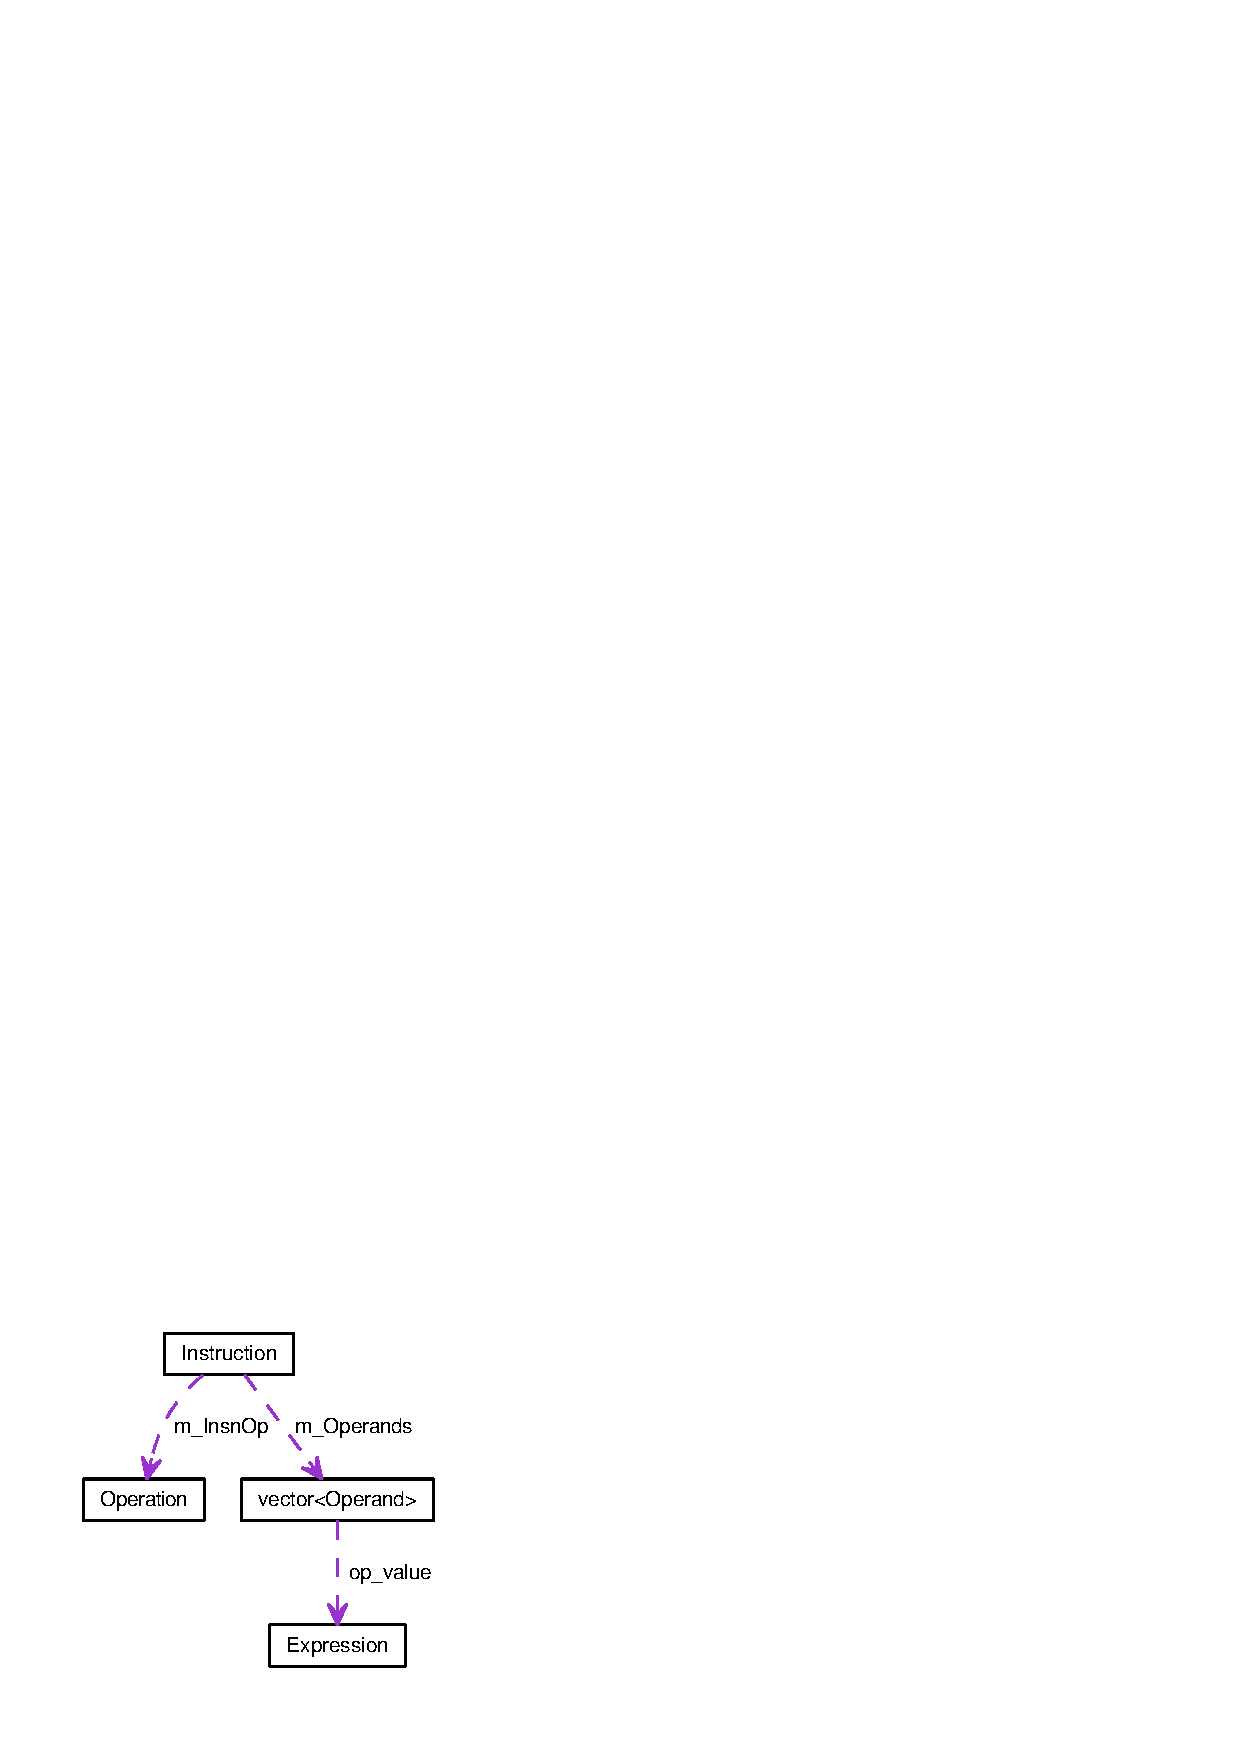
\includegraphics{ownership_graph}
\caption{An Instruction and the objects it owns}
\end{DoxyImage}
 Instruction objects provide two types of interfaces: direct read access to their components, and common summary operations on those components. The first interface allows access to the Operation and Operand data members, and each Operand object in turn allows traversal of its abstract syntax tree. More details about how to work with this abstract syntax tree can be found in \doxyref{InstructionAST Hierarchy}{p.}{group__instruction__ast__module}. This interface would be used, for example, in a data flow analysis where a user wants to evaluate the results of an effective address computation given a known register state.

The second interface allows a user to get the sets of registers read and written by the instruction, information about how the instruction accesses memory, and information about how the instruction affects control flow, without having to manipulate the Operands directly. For instance, a user could implement a register liveness analysis algorithm using just this second interface (namely the {\ttfamily getReadSet} and {\ttfamily getWriteSet} functions). 
\subsection{Instruction Decoding}
\label{group__instructiondecoder}\index{Instruction Decoding@{Instruction Decoding}}
An InstructionDecoder interprets a sequence of bytes according to a given machine language and transforms them into an instruction representation. It determines the opcode of the machine instruction, translates that opcode to an Operation object, uses that Operation to determine how to decode the instruction's Operands, and produces a decoded Instruction.


\begin{DoxyImage}
\includegraphics{decoder_use}
\caption{The InstructionDecoder's inputs and outputs}
\end{DoxyImage}
 Instruction decoders are built from the following elements:
\begin{DoxyItemize}
\item A function to find and extract an opcode given a pointer into a buffer that points to the beginning of a machine instruction
\item A table that, for a particular architecture, maps opcodes to Operations and functions that decode Operands
\end{DoxyItemize}

From these elements, it is possible to generalize the construction of Instructions from Operations and Operands to an entirely platform-\/independent algorithm. Likewise, much of the construction of the ASTs representing each operand can be performed in a platform-\/independent manner. 
\subsection{InstructionAST Hierarchy}
\label{group__instruction__ast__module}\index{InstructionAST Hierarchy@{InstructionAST Hierarchy}}
The AST representation of an operand encapsulates the operations performed on registers and immediates to produce an operand for the machine language instruction.

The inheritance hierarchy of the AST classes is shown in Figure 3. 
\begin{DoxyImage}
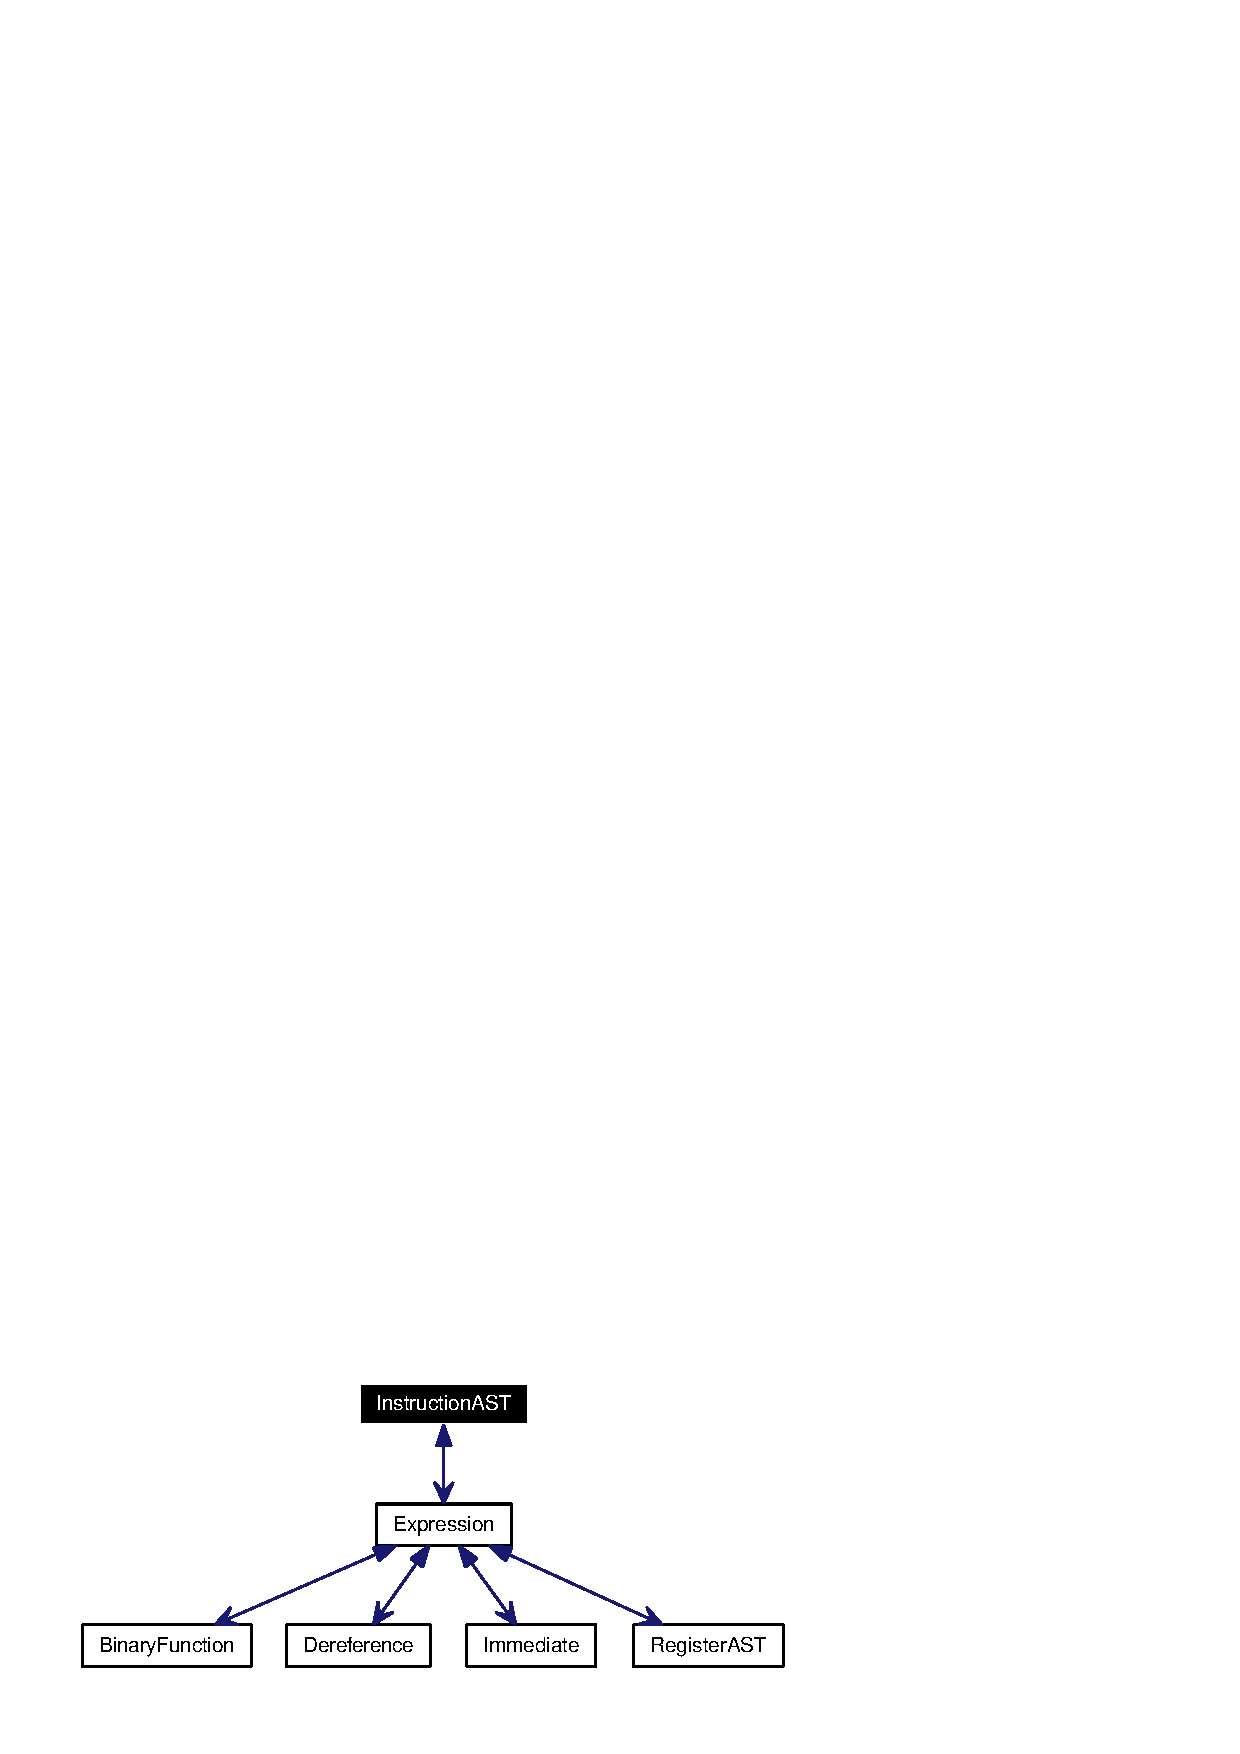
\includegraphics{full_inheritance_graph}
\caption{The InstructionAST inheritance hierarchy}
\end{DoxyImage}
 The grammar for these AST representations is simple: all leaves must be RegisterAST or Immediate nodes. These nodes may be combined using a BinaryFunction node, which may be constructed as either an addition or a multiplication. Also, a single node may descend from a Dereference node, which treats its child as a memory address. Figure 4 shows the allowable parent/child relationships within a given tree, and Figure 5 shows how an example IA32 instruction is represented using these objects. 
\begin{DoxyImage}
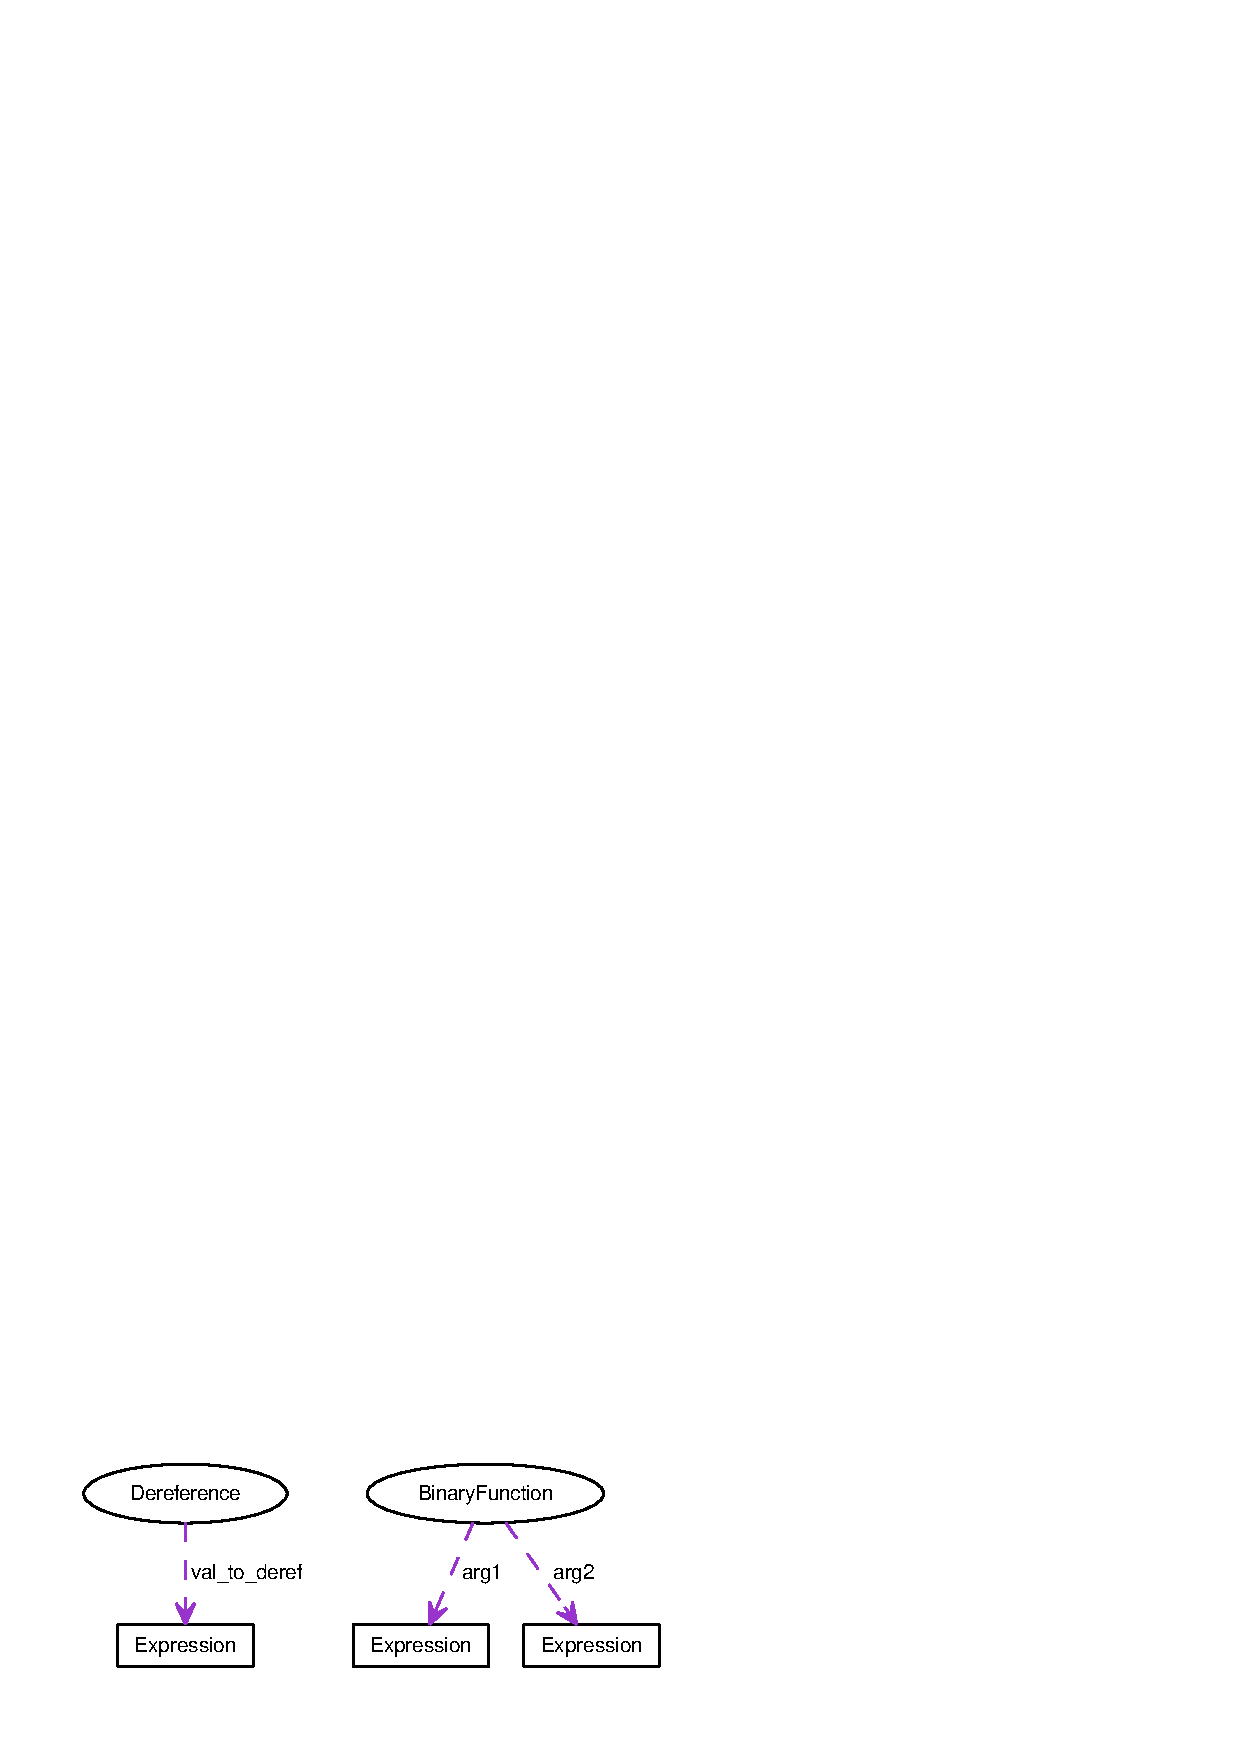
\includegraphics{ast_ownership}
\caption{InstructionAST intermediate node types and the objects they own}
\end{DoxyImage}
 
\begin{DoxyImage}
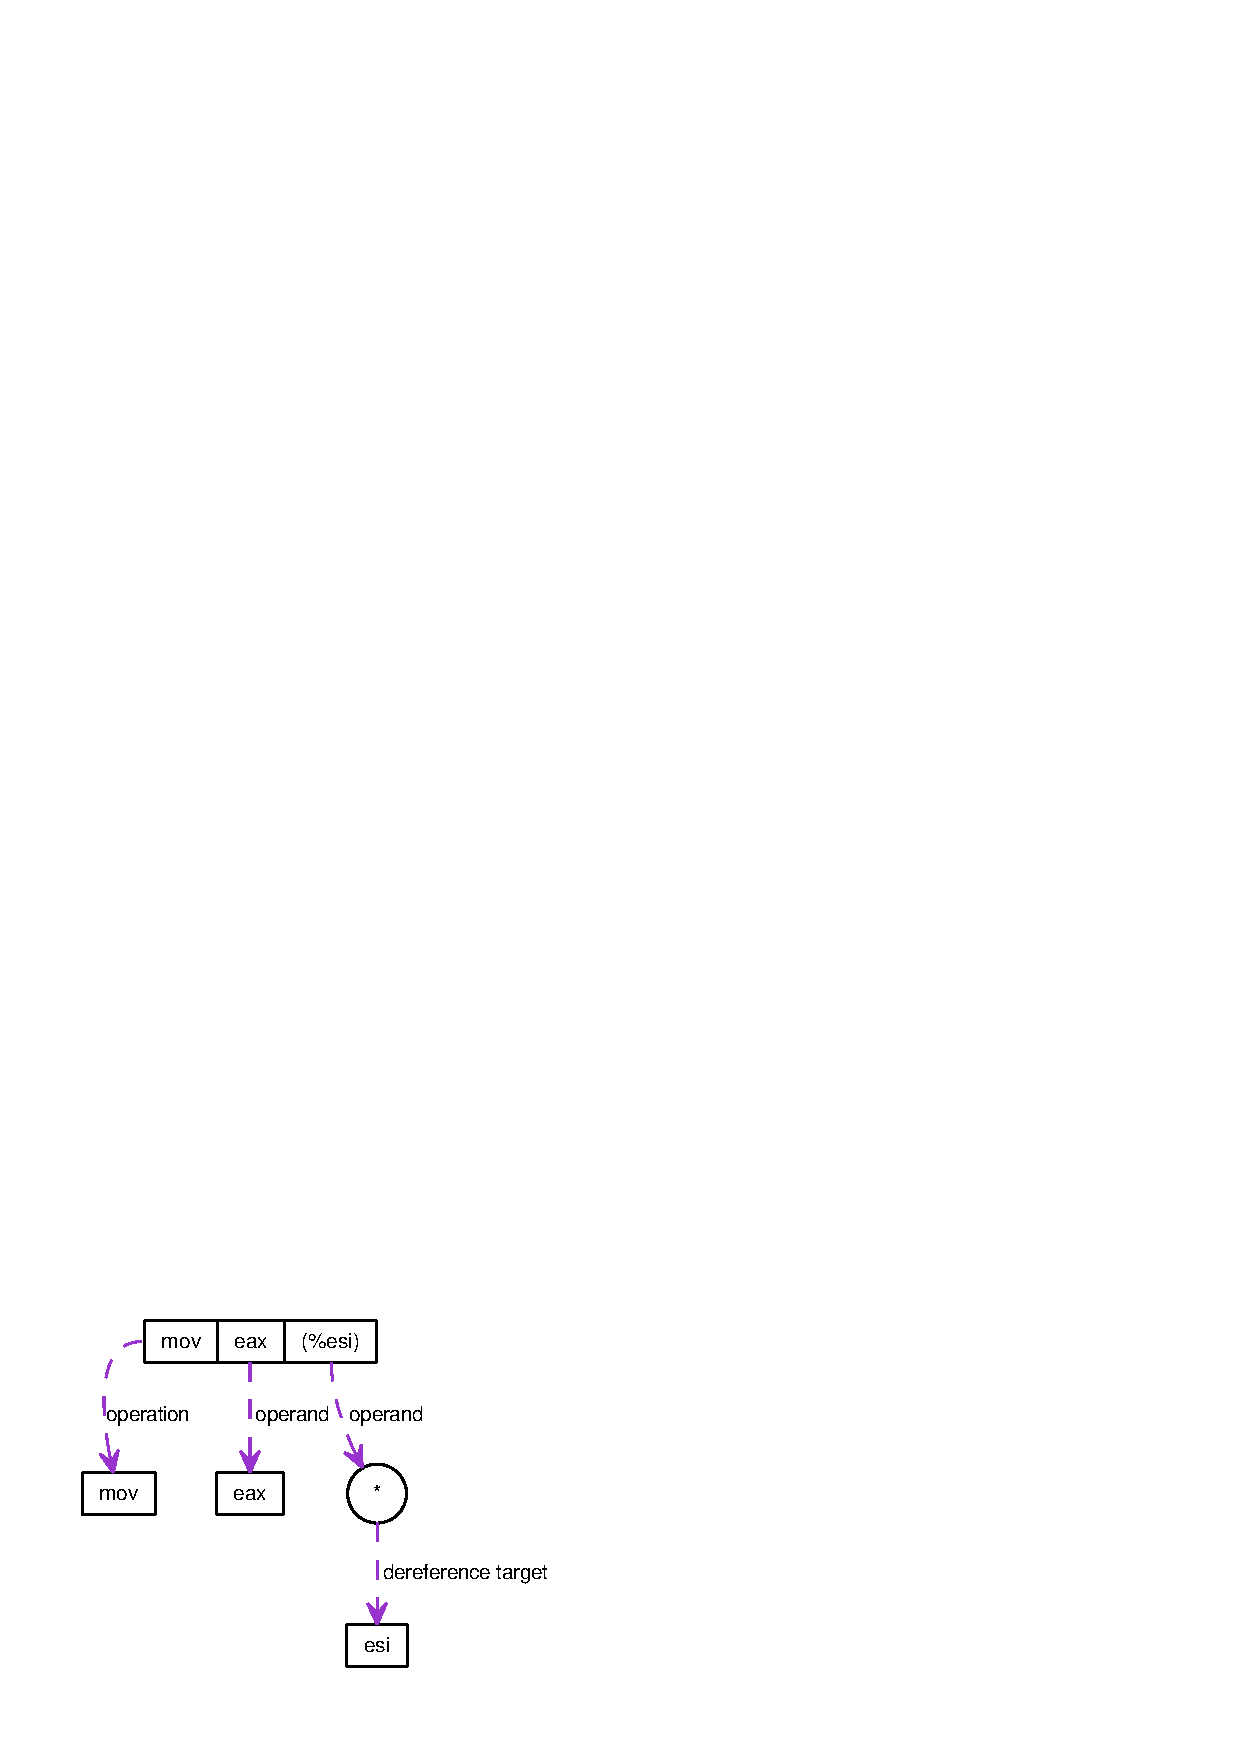
\includegraphics{instruction_representation}
\caption{The decomposition of {\ttfamily mov} {\ttfamily \%eax}, ({\ttfamily \%esi})}
\end{DoxyImage}
 These ASTs may be searched for leaf elements or subtrees (via {\ttfamily getUses} and {\ttfamily isUsed}) and traversed breadth-\/first or depth-\/first (via {\ttfamily getChildren}).

Any node in these ASTs may be evaluated. Evaluation attempts to determine the value represented by a node. If successful, it will return that value and cache it in the node. The tree structure, combined with the evaluation mechanism, allows the substitution of known register and memory values into an operand, regardless of whether those values are known at the time an instruction is decoded. More details on this mechanism may be found in \doxyref{Dyninst::InstructionAPI::Expression}{p.}{classDyninst_1_1InstructionAPI_1_1Expression}. 
\section{Class Reference}
\subsection{Instruction Class}
\label{classDyninst_1_1InstructionAPI_1_1Instruction}\index{Dyninst::InstructionAPI::Instruction@{Dyninst::InstructionAPI::Instruction}}
\subsubsection*{Public Member Functions}
\begin{DoxyCompactItemize}
\item 
 {\textbf Instruction} (Operation::Ptr what, size\_\-t size, const unsigned char $\ast$raw, Dyninst::Architecture arch)
\item 
 const {\textbf Operation} \& {\textbf getOperation} () const 
\item 
 void {\textbf getOperands} (std::vector$<$ {\textbf Operand} $>$ \&operands) const 
\item 
 {\textbf Operand} {\textbf getOperand} (int index) const 
\item 
 unsigned char {\textbf rawByte} (unsigned int index) const 
\item 
 const void $\ast$ {\textbf ptr} () const 
\item 
 void {\textbf getWriteSet} (std::set$<$ {\textbf RegisterAST::Ptr} $>$ \&regsWritten) const 
\item 
 void {\textbf getReadSet} (std::set$<$ {\textbf RegisterAST::Ptr} $>$ \&regsRead) const 
\item 
 bool {\textbf isRead} ({\textbf Expression::Ptr} candidate) const 
\item 
 bool {\textbf isWritten} ({\textbf Expression::Ptr} candidate) const 
\item 
 bool {\textbf readsMemory} () const 
\item 
 bool {\textbf writesMemory} () const 
\item 
 void {\textbf getMemoryReadOperands} (std::set$<$ {\textbf Expression::Ptr} $>$ \&memAccessors) const 
\item 
 void {\textbf getMemoryWriteOperands} (std::set$<$ {\textbf Expression::Ptr} $>$ \&memAccessors) const 
\item 
 {\textbf Expression::Ptr} {\textbf getControlFlowTarget} () const 
\item 
 bool {\textbf allowsFallThrough} () const 
\item 
 std::string {\textbf format} (Address addr=0) const 
\item 
 bool {\textbf isValid} () const 
\item 
 bool {\textbf isLegalInsn} () const 
\item 
 InsnCategory {\textbf getCategory} () const 
\end{DoxyCompactItemize}



The Instruction class is a generic instruction representation that contains operands, read/write semantic information about those operands, and information about what other registers and memory locations are affected by the operation the instruction performs.

The purpose of an Instruction object is to join an Operation with a sequence of Operands, and provide an interface for some common summary analyses (namely, the read/write sets, memory access information, and control flow information).

The Operation contains knowledge about its mnemonic and sufficient semantic details to answer the following questions:
\begin{DoxyItemize}
\item What Operands are read/written?
\item What registers are implicitly read/written?
\item What memory locations are implicitly read/written?
\item What are the possible control flow successors of this instruction?
\end{DoxyItemize}

Each Operand is an AST built from RegisterAST and Immediate leaves. For each Operand, you may determine:
\begin{DoxyItemize}
\item Registers read
\item Registers written
\item Whether memory is read or written
\item Which memory addresses are read or written, given the state of all relevant registers
\end{DoxyItemize}

Instructions should be constructed from an {\ttfamily unsigned} {\ttfamily char$\ast$} pointing to machine language, using the InstructionDecoder class. See InstructionDecoder for more details. 

\subsubsection{Constructors \& Destructors}
\index{Dyninst::InstructionAPI::Instruction@{Dyninst::InstructionAPI::Instruction}!Instruction@{Instruction}}
\index{Instruction@{Instruction}!Dyninst::InstructionAPI::Instruction@{Dyninst::InstructionAPI::Instruction}}
\paragraph[{Instruction}]{\setlength{\rightskip}{0pt plus 5cm} {\textbf Instruction} (
\begin{DoxyParamCaption}
\item[{Operation::Ptr}]{ what, }
\item[{size\_\-t}]{ size, }
\item[{const unsigned char $\ast$}]{ raw, }
\item[{Dyninst::Architecture}]{ arch}
\end{DoxyParamCaption}
)}\hfill\label{classDyninst_1_1InstructionAPI_1_1Instruction_ab02bfda322f85f88b9552681e0286362}

\begin{DoxyParams}{Parameters}
\item[{\em what}]Opcode of the instruction \item[{\em operandSource}]Contains the Expressions to be transformed into Operands \item[{\em size}]Contains the number of bytes occupied by the corresponding machine instruction \item[{\em raw}]Contains a pointer to the buffer from which this instruction object was decoded.\end{DoxyParams}
Construct an Instruction from an Operation and a collection of Expressions. This method is not intended to be used except by the InstructionDecoder class, which serves as a factory class for producing Instruction objects. While an Instruction object may be built \char`\"{}by hand\char`\"{} if desired, using the decoding interface ensures that the operation and operands are a sensible combination, and that the size reported is based on the actual size of a legal encoding of the machine instruction represented. In the course of constructing an Instruction, the Expressions in {\ttfamily operandSource} will be transformed to Operand objects. This transformation will map the semantic information about which operands are read and written in the Operation object {\ttfamily what} to the value computations in {\ttfamily operandSource}. 

\subsubsection{Member Functions}
\index{Dyninst::InstructionAPI::Instruction@{Dyninst::InstructionAPI::Instruction}!getOperation@{getOperation}}
\index{getOperation@{getOperation}!Dyninst::InstructionAPI::Instruction@{Dyninst::InstructionAPI::Instruction}}
\paragraph[{getOperation}]{\setlength{\rightskip}{0pt plus 5cm} const {\textbf Operation} \& getOperation (
\begin{DoxyParamCaption}
{}
\end{DoxyParamCaption}
) const}\hfill\label{classDyninst_1_1InstructionAPI_1_1Instruction_a1f88b414cacba47b4b66405add6ff83f}
\begin{DoxyReturn}{Returns}
The Operation used by the Instruction
\end{DoxyReturn}
See \doxyref{Operation}{p.}{classDyninst_1_1InstructionAPI_1_1Operation} for details of the Operation interface. \index{Dyninst::InstructionAPI::Instruction@{Dyninst::InstructionAPI::Instruction}!getOperands@{getOperands}}
\index{getOperands@{getOperands}!Dyninst::InstructionAPI::Instruction@{Dyninst::InstructionAPI::Instruction}}
\paragraph[{getOperands}]{\setlength{\rightskip}{0pt plus 5cm} void getOperands (
\begin{DoxyParamCaption}
\item[{std::vector$<$ {\textbf Operand} $>$ \&}]{ operands}
\end{DoxyParamCaption}
) const}\hfill\label{classDyninst_1_1InstructionAPI_1_1Instruction_a6c32c683dbd7490f18c071a648cad65b}
The vector {\ttfamily operands} has the instruction's operands appended to it in the same order that they were decoded. \index{Dyninst::InstructionAPI::Instruction@{Dyninst::InstructionAPI::Instruction}!getOperand@{getOperand}}
\index{getOperand@{getOperand}!Dyninst::InstructionAPI::Instruction@{Dyninst::InstructionAPI::Instruction}}
\paragraph[{getOperand}]{\setlength{\rightskip}{0pt plus 5cm} {\textbf Operand} getOperand (
\begin{DoxyParamCaption}
\item[{int}]{ index}
\end{DoxyParamCaption}
) const}\hfill\label{classDyninst_1_1InstructionAPI_1_1Instruction_a547bf131b520ffdc559726d27d2ced9d}
The {\ttfamily getOperand} method returns the operand at position {\ttfamily index}, or an empty operand if {\ttfamily index} does not correspond to a valid operand in this instruction. \index{Dyninst::InstructionAPI::Instruction@{Dyninst::InstructionAPI::Instruction}!rawByte@{rawByte}}
\index{rawByte@{rawByte}!Dyninst::InstructionAPI::Instruction@{Dyninst::InstructionAPI::Instruction}}
\paragraph[{rawByte}]{\setlength{\rightskip}{0pt plus 5cm} unsigned char rawByte (
\begin{DoxyParamCaption}
\item[{unsigned int}]{ index}
\end{DoxyParamCaption}
) const}\hfill\label{classDyninst_1_1InstructionAPI_1_1Instruction_a4346d867f708c491bc4218025cceb343}
Returns a pointer to the buffer from which this instruction was decoded. \index{Dyninst::InstructionAPI::Instruction@{Dyninst::InstructionAPI::Instruction}!ptr@{ptr}}
\index{ptr@{ptr}!Dyninst::InstructionAPI::Instruction@{Dyninst::InstructionAPI::Instruction}}
\paragraph[{ptr}]{\setlength{\rightskip}{0pt plus 5cm} const void $\ast$ ptr (
\begin{DoxyParamCaption}
{}
\end{DoxyParamCaption}
) const}\hfill\label{classDyninst_1_1InstructionAPI_1_1Instruction_a86f16baf5d6a6e3c0fbe392961d9a59b}
Returns a pointer to the raw byte representation of the corresponding machine instruction. \index{Dyninst::InstructionAPI::Instruction@{Dyninst::InstructionAPI::Instruction}!getWriteSet@{getWriteSet}}
\index{getWriteSet@{getWriteSet}!Dyninst::InstructionAPI::Instruction@{Dyninst::InstructionAPI::Instruction}}
\paragraph[{getWriteSet}]{\setlength{\rightskip}{0pt plus 5cm} void getWriteSet (
\begin{DoxyParamCaption}
\item[{std::set$<$ {\textbf RegisterAST::Ptr} $>$ \&}]{ regsWritten}
\end{DoxyParamCaption}
) const}\hfill\label{classDyninst_1_1InstructionAPI_1_1Instruction_aabb2d82e550db2a060fd490b6a554527}

\begin{DoxyParams}{Parameters}
\item[{\em regsWritten}]Insert the set of registers written by the instruction into {\ttfamily regsWritten}.\end{DoxyParams}
The list of registers returned in {\ttfamily regsWritten} includes registers that are explicitly written as destination operands (like the destination of a move). It also includes registers that are implicitly written (like the stack pointer in a push or pop instruction). It does not include any registers used only in computing the effective address of a write. {\ttfamily pop} {\ttfamily $\ast$eax}, for example, writes to {\ttfamily esp}, reads {\ttfamily esp}, and reads {\ttfamily eax}, but despite the fact that {\ttfamily $\ast$eax} is the destination operand, {\ttfamily eax} is not itself written.

For both the write set and the read set (below), it is possible to determine whether a register is accessed implicitly or explicitly by examining the Operands. An explicitly accessed register appears as an operand that is written or read; also, any registers used in any address calculations are explicitly read. Any element of the write set or read set that is not explicitly written or read is implicitly written or read. \index{Dyninst::InstructionAPI::Instruction@{Dyninst::InstructionAPI::Instruction}!getReadSet@{getReadSet}}
\index{getReadSet@{getReadSet}!Dyninst::InstructionAPI::Instruction@{Dyninst::InstructionAPI::Instruction}}
\paragraph[{getReadSet}]{\setlength{\rightskip}{0pt plus 5cm} void getReadSet (
\begin{DoxyParamCaption}
\item[{std::set$<$ {\textbf RegisterAST::Ptr} $>$ \&}]{ regsRead}
\end{DoxyParamCaption}
) const}\hfill\label{classDyninst_1_1InstructionAPI_1_1Instruction_af6d94aa7ad62e7d980a3bbf2b850c4fa}

\begin{DoxyParams}{Parameters}
\item[{\em regsRead}]Insert the set of registers read by the instruction into {\ttfamily regsRead}.\end{DoxyParams}
If an operand is used to compute an effective address, the registers involved are read but not written, regardless of the effect on the operand. \index{Dyninst::InstructionAPI::Instruction@{Dyninst::InstructionAPI::Instruction}!isRead@{isRead}}
\index{isRead@{isRead}!Dyninst::InstructionAPI::Instruction@{Dyninst::InstructionAPI::Instruction}}
\paragraph[{isRead}]{\setlength{\rightskip}{0pt plus 5cm} bool isRead (
\begin{DoxyParamCaption}
\item[{{\textbf Expression::Ptr}}]{ candidate}
\end{DoxyParamCaption}
) const}\hfill\label{classDyninst_1_1InstructionAPI_1_1Instruction_a2ddfb452ef7992b8698b4173a52d2d46}

\begin{DoxyParams}{Parameters}
\item[{\em candidate}]Subexpression to search for among the values read by this Instruction object.\end{DoxyParams}
Returns true if {\ttfamily candidate} is read by this Instruction. \index{Dyninst::InstructionAPI::Instruction@{Dyninst::InstructionAPI::Instruction}!isWritten@{isWritten}}
\index{isWritten@{isWritten}!Dyninst::InstructionAPI::Instruction@{Dyninst::InstructionAPI::Instruction}}
\paragraph[{isWritten}]{\setlength{\rightskip}{0pt plus 5cm} bool isWritten (
\begin{DoxyParamCaption}
\item[{{\textbf Expression::Ptr}}]{ candidate}
\end{DoxyParamCaption}
) const}\hfill\label{classDyninst_1_1InstructionAPI_1_1Instruction_ac7703dd7bef37d76420e74e2811ebef6}

\begin{DoxyParams}{Parameters}
\item[{\em candidate}]Subexpression to search for among the values written by this Instruction object.\end{DoxyParams}
Returns true if {\ttfamily candidate} is written by this Instruction. \index{Dyninst::InstructionAPI::Instruction@{Dyninst::InstructionAPI::Instruction}!readsMemory@{readsMemory}}
\index{readsMemory@{readsMemory}!Dyninst::InstructionAPI::Instruction@{Dyninst::InstructionAPI::Instruction}}
\paragraph[{readsMemory}]{\setlength{\rightskip}{0pt plus 5cm} bool readsMemory (
\begin{DoxyParamCaption}
{}
\end{DoxyParamCaption}
) const}\hfill\label{classDyninst_1_1InstructionAPI_1_1Instruction_a093a3808c1e3569807dfc42de72d15de}
\begin{DoxyReturn}{Returns}
Returns true if the instruction reads at least one memory address as data.
\end{DoxyReturn}
If any operand containing a Dereference object is read, the instruction reads the memory at that address. Also, on platforms where a stack pop is guaranteed to read memory, {\ttfamily readsMemory} will return true for a pop operation. \index{Dyninst::InstructionAPI::Instruction@{Dyninst::InstructionAPI::Instruction}!writesMemory@{writesMemory}}
\index{writesMemory@{writesMemory}!Dyninst::InstructionAPI::Instruction@{Dyninst::InstructionAPI::Instruction}}
\paragraph[{writesMemory}]{\setlength{\rightskip}{0pt plus 5cm} bool writesMemory (
\begin{DoxyParamCaption}
{}
\end{DoxyParamCaption}
) const}\hfill\label{classDyninst_1_1InstructionAPI_1_1Instruction_a66f951a83dd868bac2d0b69625da6f8a}
\begin{DoxyReturn}{Returns}
Returns true if the instruction writes at least one memory address.
\end{DoxyReturn}
If any operand containing a Dereference object is written, the instruction writes the memory at that address. Also, on platforms where a stack push is guaranteed to write memory, {\ttfamily writesMemory} will return true for a push operation. \index{Dyninst::InstructionAPI::Instruction@{Dyninst::InstructionAPI::Instruction}!getMemoryReadOperands@{getMemoryReadOperands}}
\index{getMemoryReadOperands@{getMemoryReadOperands}!Dyninst::InstructionAPI::Instruction@{Dyninst::InstructionAPI::Instruction}}
\paragraph[{getMemoryReadOperands}]{\setlength{\rightskip}{0pt plus 5cm} void getMemoryReadOperands (
\begin{DoxyParamCaption}
\item[{std::set$<$ {\textbf Expression::Ptr} $>$ \&}]{ memAccessors}
\end{DoxyParamCaption}
) const}\hfill\label{classDyninst_1_1InstructionAPI_1_1Instruction_a01b2e0d9786ff3e44ac6fec4f9d098fa}

\begin{DoxyParams}{Parameters}
\item[{\em memAccessors}]Addresses read by this instruction are inserted into {\ttfamily memAccessors} \end{DoxyParams}
The addresses read are in the form of Expressions, which may be evaluated once all of the registers that they use have had their values set. Note that this method returns ASTs representing address computations, and not address accesses. For instance, an instruction accessing memory through a register dereference would return a Expression tree containing just the register that determines the address being accessed, not a tree representing a dereference of that register. \index{Dyninst::InstructionAPI::Instruction@{Dyninst::InstructionAPI::Instruction}!getMemoryWriteOperands@{getMemoryWriteOperands}}
\index{getMemoryWriteOperands@{getMemoryWriteOperands}!Dyninst::InstructionAPI::Instruction@{Dyninst::InstructionAPI::Instruction}}
\paragraph[{getMemoryWriteOperands}]{\setlength{\rightskip}{0pt plus 5cm} void getMemoryWriteOperands (
\begin{DoxyParamCaption}
\item[{std::set$<$ {\textbf Expression::Ptr} $>$ \&}]{ memAccessors}
\end{DoxyParamCaption}
) const}\hfill\label{classDyninst_1_1InstructionAPI_1_1Instruction_ac86abff921a298797619ed078b75f6fd}

\begin{DoxyParams}{Parameters}
\item[{\em memAccessors}]Addresses written by this instruction are inserted into {\ttfamily memAccessors} \end{DoxyParams}
The addresses written are in the same form as those returned by {\ttfamily getMemoryReadOperands} above. \index{Dyninst::InstructionAPI::Instruction@{Dyninst::InstructionAPI::Instruction}!getControlFlowTarget@{getControlFlowTarget}}
\index{getControlFlowTarget@{getControlFlowTarget}!Dyninst::InstructionAPI::Instruction@{Dyninst::InstructionAPI::Instruction}}
\paragraph[{getControlFlowTarget}]{\setlength{\rightskip}{0pt plus 5cm} {\textbf Expression::Ptr} getControlFlowTarget (
\begin{DoxyParamCaption}
{}
\end{DoxyParamCaption}
) const}\hfill\label{classDyninst_1_1InstructionAPI_1_1Instruction_a767e00b187b1a5287e82d26b816d6efe}
\begin{DoxyReturn}{Returns}
An expression evaluating to the non-\/fallthrough control flow targets, if any, of this instruction.
\end{DoxyReturn}
When called on an explicitly control-\/flow altering instruction, returns the non-\/fallthrough control flow destination. When called on any other instruction, returns {\ttfamily NULL}.

For direct absolute branch instructions, {\ttfamily getControlFlowTarget} will return an immediate value. For direct relative branch instructions, {\ttfamily getControlFlowTarget} will return the expression {\ttfamily PC} + offset. In the case of indirect branches and calls, it returns a dereference of a register (or possibly a dereference of a more complicated expression). In this case, data flow analysis will often allow the determination of the possible targets of the instruction. We do not do analysis beyond the single-\/instruction level in the Instruction API; if other code performs this type of analysis, it may update the information in the Dereference object using the setValue method in the Expression interface. More details about this may be found in \doxyref{Expression}{p.}{classDyninst_1_1InstructionAPI_1_1Expression} and \doxyref{Dereference}{p.}{classDyninst_1_1InstructionAPI_1_1Dereference}. \index{Dyninst::InstructionAPI::Instruction@{Dyninst::InstructionAPI::Instruction}!allowsFallThrough@{allowsFallThrough}}
\index{allowsFallThrough@{allowsFallThrough}!Dyninst::InstructionAPI::Instruction@{Dyninst::InstructionAPI::Instruction}}
\paragraph[{allowsFallThrough}]{\setlength{\rightskip}{0pt plus 5cm} bool allowsFallThrough (
\begin{DoxyParamCaption}
{}
\end{DoxyParamCaption}
) const}\hfill\label{classDyninst_1_1InstructionAPI_1_1Instruction_ab67a3a8783e0f74532c46ac0026e5659}
\begin{DoxyReturn}{Returns}
False if control flow will unconditionally go to the result of {\ttfamily getControlFlowTarget} after executing this instruction. 
\end{DoxyReturn}
\index{Dyninst::InstructionAPI::Instruction@{Dyninst::InstructionAPI::Instruction}!format@{format}}
\index{format@{format}!Dyninst::InstructionAPI::Instruction@{Dyninst::InstructionAPI::Instruction}}
\paragraph[{format}]{\setlength{\rightskip}{0pt plus 5cm} std::string format (
\begin{DoxyParamCaption}
\item[{Address}]{ addr = {\ttfamily 0}}
\end{DoxyParamCaption}
) const}\hfill\label{classDyninst_1_1InstructionAPI_1_1Instruction_a9e3720c9fc28a4ef520ac6e2a106b6fa}
\begin{DoxyReturn}{Returns}
The instruction as a string of assembly language
\end{DoxyReturn}
{\ttfamily format} is principally a helper function; Instructions are meant to be written to output streams via {\ttfamily operator$<$$<$}. {\ttfamily format} is included in the public interface for diagnostic purposes. \index{Dyninst::InstructionAPI::Instruction@{Dyninst::InstructionAPI::Instruction}!isValid@{isValid}}
\index{isValid@{isValid}!Dyninst::InstructionAPI::Instruction@{Dyninst::InstructionAPI::Instruction}}
\paragraph[{isValid}]{\setlength{\rightskip}{0pt plus 5cm} bool isValid (
\begin{DoxyParamCaption}
{}
\end{DoxyParamCaption}
) const}\hfill\label{classDyninst_1_1InstructionAPI_1_1Instruction_a99a5165ae8b791c61ef8be354f2e8b78}
Returns true if this Instruction object is valid. Invalid instructions indicate that an InstructionDecoder has reached the end of its assigned range, and that decoding should terminate. \index{Dyninst::InstructionAPI::Instruction@{Dyninst::InstructionAPI::Instruction}!isLegalInsn@{isLegalInsn}}
\index{isLegalInsn@{isLegalInsn}!Dyninst::InstructionAPI::Instruction@{Dyninst::InstructionAPI::Instruction}}
\paragraph[{isLegalInsn}]{\setlength{\rightskip}{0pt plus 5cm} bool isLegalInsn (
\begin{DoxyParamCaption}
{}
\end{DoxyParamCaption}
) const}\hfill\label{classDyninst_1_1InstructionAPI_1_1Instruction_a3ad6500b0772392139a156898a236ea0}
Returns true if this Instruction object represents a legal instruction, as specified by the architecture used to decode this instruction. \index{Dyninst::InstructionAPI::Instruction@{Dyninst::InstructionAPI::Instruction}!getCategory@{getCategory}}
\index{getCategory@{getCategory}!Dyninst::InstructionAPI::Instruction@{Dyninst::InstructionAPI::Instruction}}
\paragraph[{getCategory}]{\setlength{\rightskip}{0pt plus 5cm} InsnCategory getCategory (
\begin{DoxyParamCaption}
{}
\end{DoxyParamCaption}
) const}\hfill\label{classDyninst_1_1InstructionAPI_1_1Instruction_a1bf11a5bf394b394f3e89cdc7bf8f616}
ALPHA: Returns the category that an instruction falls into. This feature is presently incomplete, and we welcome feedback on ways to extend it usefully.

Currently, the valid categories are c\_\-CallInsn, c\_\-ReturnInsn, c\_\-BranchInsn, c\_\-CompareInsn, and c\_\-NoCategory, as defined in InstructionCategories.h. 
\subsection{Operation Class}
\label{classDyninst_1_1InstructionAPI_1_1Operation}\index{Dyninst::InstructionAPI::Operation@{Dyninst::InstructionAPI::Operation}}
\subsubsection*{Public Member Functions}
\begin{DoxyCompactItemize}
\item 
 std::string {\textbf format} () const 
\item 
 entryID {\textbf getID} () const 
\item 
 prefixEntryID {\textbf getPrefixID} () const 
\end{DoxyCompactItemize}



An Operation object represents a family of opcodes (operation encodings) that perform the same task (e.g. the {\ttfamily MOV} family). It includes information about the number of operands, their read/write semantics, the implicit register reads and writes, and the control flow behavior of a particular assembly language operation. It additionally provides access to the assembly mnemonic, which allows any semantic details that are not encoded in the Instruction representation to be added by higher layers of analysis.

As an example, the {\ttfamily CMP} operation on IA32/AMD64 processors has the following properties:
\begin{DoxyItemize}
\item Operand 1 is read, but not written
\item Operand 2 is read, but not written
\item The following flags are written:
\begin{DoxyItemize}
\item Overflow
\item Sign
\item Zero
\item Parity
\item Carry
\item Auxiliary
\end{DoxyItemize}
\item No other registers are read, and no implicit memory operations are performed
\end{DoxyItemize}

Operations are constructed by the InstructionDecoder as part of the process of constructing an Instruction. 

\subsubsection{Member Functions}
\index{Dyninst::InstructionAPI::Operation@{Dyninst::InstructionAPI::Operation}!format@{format}}
\index{format@{format}!Dyninst::InstructionAPI::Operation@{Dyninst::InstructionAPI::Operation}}
\paragraph[{format}]{\setlength{\rightskip}{0pt plus 5cm}std::string format (
\begin{DoxyParamCaption}
{}
\end{DoxyParamCaption}
) const}\hfill\label{classDyninst_1_1InstructionAPI_1_1Operation_a204c75f752ee13cb64ccc2b7af3f687c}
Returns the mnemonic for the operation. Like {\ttfamily instruction::format}, this is exposed for debugging and will be replaced with stream operators in the public interface. \index{Dyninst::InstructionAPI::Operation@{Dyninst::InstructionAPI::Operation}!getID@{getID}}
\index{getID@{getID}!Dyninst::InstructionAPI::Operation@{Dyninst::InstructionAPI::Operation}}
\paragraph[{getID}]{\setlength{\rightskip}{0pt plus 5cm}entryID getID (
\begin{DoxyParamCaption}
{}
\end{DoxyParamCaption}
) const}\hfill\label{classDyninst_1_1InstructionAPI_1_1Operation_a36f4818569bf4881244ab4a4c7f2ba06}
Returns the entry ID corresponding to this operation. Entry IDs are enumerated values that correspond to assembly mnemonics. \index{Dyninst::InstructionAPI::Operation@{Dyninst::InstructionAPI::Operation}!getPrefixID@{getPrefixID}}
\index{getPrefixID@{getPrefixID}!Dyninst::InstructionAPI::Operation@{Dyninst::InstructionAPI::Operation}}
\paragraph[{getPrefixID}]{\setlength{\rightskip}{0pt plus 5cm}prefixEntryID getPrefixID (
\begin{DoxyParamCaption}
{}
\end{DoxyParamCaption}
) const}\hfill\label{classDyninst_1_1InstructionAPI_1_1Operation_a8ae500d97f21b771c252a6814fcf5c4a}
Returns the prefix entry ID corresponding to this operation, if any. Prefix IDs are enumerated values that correspond to assembly prefix mnemonics. 
\subsection{Operand Class}
\label{classDyninst_1_1InstructionAPI_1_1Operand}\index{Dyninst::InstructionAPI::Operand@{Dyninst::InstructionAPI::Operand}}
\subsubsection*{Public Member Functions}
\begin{DoxyCompactItemize}
\item 
{\textbf Operand} ({\textbf Expression::Ptr} val, bool read, bool written)
\item 
 void {\textbf getReadSet} (std::set$<$ {\textbf RegisterAST::Ptr} $>$ \&regsRead) const 
\item 
 void {\textbf getWriteSet} (std::set$<$ {\textbf RegisterAST::Ptr} $>$ \&regsWritten) const 
\item 
 void {\textbf addEffectiveReadAddresses} (std::set$<$ {\textbf Expression::Ptr} $>$ \&memAccessors) const 
\item 
 void {\textbf addEffectiveWriteAddresses} (std::set$<$ {\textbf Expression::Ptr} $>$ \&memAccessors) const 
\item 
 std::string {\textbf format} (Architecture arch, Address addr=0) const 
\end{DoxyCompactItemize}



An Operand object contains an AST built from RegisterAST and Immediate leaves, and information about whether the Operand is read, written, or both. This allows us to determine which of the registers that appear in the Operand are read and which are written, as well as whether any memory accesses are reads, writes, or both. An Operand, given full knowledge of the values of the leaves of the AST, and knowledge of the logic associated with the tree's internal nodes, can determine the result of any computations that are encoded in it. It will rarely be the case that an Instruction is built with its Operands' state fully specified. This mechanism is instead intended to allow a user to fill in knowledge about the state of the processor at the time the Instruction is executed. 

\subsubsection{Constructors \& Destructors}
\index{Dyninst::InstructionAPI::Operand@{Dyninst::InstructionAPI::Operand}!Operand@{Operand}}
\index{Operand@{Operand}!Dyninst::InstructionAPI::Operand@{Dyninst::InstructionAPI::Operand}}
\paragraph[{Operand}]{\setlength{\rightskip}{0pt plus 5cm}{\textbf Operand} (
\begin{DoxyParamCaption}
\item[{{\textbf Expression::Ptr}}]{ val, }
\item[{bool}]{ read, }
\item[{bool}]{ written}
\end{DoxyParamCaption}
)}\hfill\label{classDyninst_1_1InstructionAPI_1_1Operand_a2e9e7385ab9ad68c0af145540186e7cf}


Create an operand from a Expression and flags describing whether the ValueComputation is read, written or both. 


\begin{DoxyParams}{Parameters}
\item[{\em val}]Reference-\/counted pointer to the Expression that will be contained in the Operand being constructed \item[{\em read}]True if this operand is read \item[{\em written}]True if this operand is written \end{DoxyParams}


\subsubsection{Member Functions}
\index{Dyninst::InstructionAPI::Operand@{Dyninst::InstructionAPI::Operand}!getReadSet@{getReadSet}}
\index{getReadSet@{getReadSet}!Dyninst::InstructionAPI::Operand@{Dyninst::InstructionAPI::Operand}}
\paragraph[{getReadSet}]{\setlength{\rightskip}{0pt plus 5cm} void getReadSet (
\begin{DoxyParamCaption}
\item[{std::set$<$ {\textbf RegisterAST::Ptr} $>$ \&}]{ regsRead}
\end{DoxyParamCaption}
) const}\hfill\label{classDyninst_1_1InstructionAPI_1_1Operand_af6d94aa7ad62e7d980a3bbf2b850c4fa}


Get the registers read by this operand. 


\begin{DoxyParams}{Parameters}
\item[{\em regsRead}]Has the registers read inserted into it \end{DoxyParams}
\index{Dyninst::InstructionAPI::Operand@{Dyninst::InstructionAPI::Operand}!getWriteSet@{getWriteSet}}
\index{getWriteSet@{getWriteSet}!Dyninst::InstructionAPI::Operand@{Dyninst::InstructionAPI::Operand}}
\paragraph[{getWriteSet}]{\setlength{\rightskip}{0pt plus 5cm} void getWriteSet (
\begin{DoxyParamCaption}
\item[{std::set$<$ {\textbf RegisterAST::Ptr} $>$ \&}]{ regsWritten}
\end{DoxyParamCaption}
) const}\hfill\label{classDyninst_1_1InstructionAPI_1_1Operand_aabb2d82e550db2a060fd490b6a554527}


Get the registers written by this operand. 


\begin{DoxyParams}{Parameters}
\item[{\em regsWritten}]Has the registers written inserted into it \end{DoxyParams}
\index{Dyninst::InstructionAPI::Operand@{Dyninst::InstructionAPI::Operand}!addEffectiveReadAddresses@{addEffectiveReadAddresses}}
\index{addEffectiveReadAddresses@{addEffectiveReadAddresses}!Dyninst::InstructionAPI::Operand@{Dyninst::InstructionAPI::Operand}}
\paragraph[{addEffectiveReadAddresses}]{\setlength{\rightskip}{0pt plus 5cm} void addEffectiveReadAddresses (
\begin{DoxyParamCaption}
\item[{std::set$<$ {\textbf Expression::Ptr} $>$ \&}]{ memAccessors}
\end{DoxyParamCaption}
) const}\hfill\label{classDyninst_1_1InstructionAPI_1_1Operand_a91c0c0397fa59fb0f53f9ad12526280a}


Inserts the effective addresses read by this operand into memAccessors. 


\begin{DoxyParams}{Parameters}
\item[{\em memAccessors}]If this is a memory read operand, insert the {\ttfamily ExpressionPtr} representing the address being read into {\ttfamily memAccessors}. \end{DoxyParams}
\index{Dyninst::InstructionAPI::Operand@{Dyninst::InstructionAPI::Operand}!addEffectiveWriteAddresses@{addEffectiveWriteAddresses}}
\index{addEffectiveWriteAddresses@{addEffectiveWriteAddresses}!Dyninst::InstructionAPI::Operand@{Dyninst::InstructionAPI::Operand}}
\paragraph[{addEffectiveWriteAddresses}]{\setlength{\rightskip}{0pt plus 5cm} void addEffectiveWriteAddresses (
\begin{DoxyParamCaption}
\item[{std::set$<$ {\textbf Expression::Ptr} $>$ \&}]{ memAccessors}
\end{DoxyParamCaption}
) const}\hfill\label{classDyninst_1_1InstructionAPI_1_1Operand_a8a766dfcc9aa94c08f0943ca5828dc8b}


Inserts the effective addresses written by this operand into memAccessors. 


\begin{DoxyParams}{Parameters}
\item[{\em memAccessors}]If this is a memory write operand, insert the {\ttfamily ExpressionPtr} representing the address being written into {\ttfamily memAccessors}. \end{DoxyParams}
\index{Dyninst::InstructionAPI::Operand@{Dyninst::InstructionAPI::Operand}!format@{format}}
\index{format@{format}!Dyninst::InstructionAPI::Operand@{Dyninst::InstructionAPI::Operand}}
\paragraph[{format}]{\setlength{\rightskip}{0pt plus 5cm} std::string format (
\begin{DoxyParamCaption}
\item[{Architecture}]{ arch, }
\item[{Address}]{ addr = {\ttfamily 0}}
\end{DoxyParamCaption}
) const}\hfill\label{classDyninst_1_1InstructionAPI_1_1Operand_a5e653615a522cf09bda1857a326d4e5f}


Return a printable string representation of the operand. 

\begin{DoxyReturn}{Returns}
The operand in a disassembly format 
\end{DoxyReturn}

\subsection{InstructionAST Class}
\label{classDyninst_1_1InstructionAPI_1_1InstructionAST}\index{Dyninst::InstructionAPI::InstructionAST@{Dyninst::InstructionAPI::InstructionAST}}
\subsubsection*{Public Member Functions}
\begin{DoxyCompactItemize}
\item 
bool {\textbf operator==} (const {\textbf InstructionAST} \&rhs) const 
\item 
virtual void {\textbf getUses} (set$<$ InstructionAST::Ptr $>$ \&uses)=0
\item 
virtual bool {\textbf isUsed} (InstructionAST::Ptr findMe) const =0
\item 
virtual std::string {\textbf format} (formatStyle how=defaultStyle) const =0
\end{DoxyCompactItemize}



The InstructionAST class is the base class for all nodes in the ASTs used by the Operand class. It defines the necessary interfaces for traversing and searching an abstract syntax tree representing an operand. For the purposes of searching an InstructionAST, we provide two related interfaces. The first, {\ttfamily getUses}, will return the registers that appear in a given tree. The second, {\ttfamily isUsed}, will take as input another tree and return true if that tree is a (not necessarily proper) subtree of this one. {\ttfamily isUsed} requires us to define an equality relation on these abstract syntax trees, and the equality operator is provided by the InstructionAST, with the details implemented by the classes derived from InstructionAST. Two AST nodes are equal if the following conditions hold:
\begin{DoxyItemize}
\item They are of the same type
\item If leaf nodes, they represent the same immediate value or the same register
\item If non-\/leaf nodes, they represent the same operation and their corresponding children are equal 
\end{DoxyItemize}

\subsubsection{Member Functions}
\index{Dyninst::InstructionAPI::InstructionAST@{Dyninst::InstructionAPI::InstructionAST}!operator==@{operator==}}
\index{operator==@{operator==}!Dyninst::InstructionAPI::InstructionAST@{Dyninst::InstructionAPI::InstructionAST}}
\paragraph[{operator==}]{\setlength{\rightskip}{0pt plus 5cm}bool operator== (
\begin{DoxyParamCaption}
\item[{const {\textbf InstructionAST} \&}]{ rhs}
\end{DoxyParamCaption}
) const}\hfill\label{classDyninst_1_1InstructionAPI_1_1InstructionAST_a1ab63f8949f2b386539d99512e0c0df4}
Compare two AST nodes for equality.

Non-\/leaf nodes are equal if they are of the same type and their children are equal. RegisterASTs are equal if they represent the same register. Immediates are equal if they represent the same value. \index{Dyninst::InstructionAPI::InstructionAST@{Dyninst::InstructionAPI::InstructionAST}!getUses@{getUses}}
\index{getUses@{getUses}!Dyninst::InstructionAPI::InstructionAST@{Dyninst::InstructionAPI::InstructionAST}}
\paragraph[{getUses}]{\setlength{\rightskip}{0pt plus 5cm}virtual void getUses (
\begin{DoxyParamCaption}
\item[{set$<$ InstructionAST::Ptr $>$ \&}]{ uses}
\end{DoxyParamCaption}
)\hspace{0.3cm}{\ttfamily  [pure virtual]}}\hfill\label{classDyninst_1_1InstructionAPI_1_1InstructionAST_ada04317a5cc7ccd076da203622193d24}

\begin{DoxyParams}{Parameters}
\item[{\em uses}]The use set of this node is appended to the vector {\ttfamily uses} \end{DoxyParams}
The use set of an InstructionAST is defined as follows:
\begin{DoxyItemize}
\item A RegisterAST uses itself
\item A BinaryFunction uses the use sets of its children
\item An Immediate uses nothing
\item A Dereference uses the use set of its child 
\end{DoxyItemize}


\index{Dyninst::InstructionAPI::InstructionAST@{Dyninst::InstructionAPI::InstructionAST}!isUsed@{isUsed}}
\index{isUsed@{isUsed}!Dyninst::InstructionAPI::InstructionAST@{Dyninst::InstructionAPI::InstructionAST}}
\paragraph[{isUsed}]{\setlength{\rightskip}{0pt plus 5cm}virtual bool isUsed (
\begin{DoxyParamCaption}
\item[{InstructionAST::Ptr}]{ findMe}
\end{DoxyParamCaption}
) const\hspace{0.3cm}{\ttfamily  [pure virtual]}}\hfill\label{classDyninst_1_1InstructionAPI_1_1InstructionAST_aef4487c2b00fc3a0e6e6e19e135c5b0e}
\begin{DoxyReturn}{Returns}
True if {\ttfamily findMe} is used by this AST node. 
\end{DoxyReturn}

\begin{DoxyParams}{Parameters}
\item[{\em findMe}]AST node to find in the use set of this node\end{DoxyParams}
Unlike {\ttfamily getUses}, {\ttfamily isUsed} looks for {\ttfamily findMe} as a subtree of the current tree. {\ttfamily getUses} is designed to return a minimal set of registers used in this tree, whereas {\ttfamily isUsed} is designed to allow searches for arbitrary subexpressions 


\index{Dyninst::InstructionAPI::InstructionAST@{Dyninst::InstructionAPI::InstructionAST}!format@{format}}
\index{format@{format}!Dyninst::InstructionAPI::InstructionAST@{Dyninst::InstructionAPI::InstructionAST}}
\paragraph[{format}]{\setlength{\rightskip}{0pt plus 5cm}virtual std::string format (
\begin{DoxyParamCaption}
\item[{formatStyle}]{ how = {\ttfamily defaultStyle}}
\end{DoxyParamCaption}
) const\hspace{0.3cm}{\ttfamily  [pure virtual]}}\hfill\label{classDyninst_1_1InstructionAPI_1_1InstructionAST_a19a491830d63df46ef88ca28167891a0}
The {\ttfamily format} interface returns the contents of an InstructionAST object as a string. By default, {\ttfamily \doxyref{format()}{p.}{classDyninst_1_1InstructionAPI_1_1InstructionAST_a19a491830d63df46ef88ca28167891a0}} produces assembly language. 



\subsection{Expression Class}
\label{classDyninst_1_1InstructionAPI_1_1Expression}\index{Dyninst::InstructionAPI::Expression@{Dyninst::InstructionAPI::Expression}}
\subsubsection*{Public Member Functions}
\begin{DoxyCompactItemize}
\item 
void {\textbf setValue} (const {\textbf Result} \&knownValue)
\item 
void {\textbf clearValue} ()
\item 
virtual bool {\textbf bind} ({\textbf Expression} $\ast$expr, const {\textbf Result} \&value)
\item 
virtual void {\textbf apply} (Visitor $\ast$)
\item 
virtual void {\textbf getChildren} (std::vector$<$ {\textbf Expression::Ptr} $>$ \&children) const =0
\end{DoxyCompactItemize}



An Expression is an AST representation of how the value of an operand is computed.

The Expression class extends the InstructionAST class by adding the concept of evaluation to the nodes of an InstructionAST. Evaluation attempts to determine the \doxyref{Result}{p.}{classDyninst_1_1InstructionAPI_1_1Result} of the computation that the AST being evaluated represents. It will fill in results of as many of the nodes in the tree as possible, and if full evaluation is possible, it will return the result of the computation performed by the tree.

Permissible leaf nodes of a Expression tree are RegisterAST and Immediate objects. Permissible internal nodes are BinaryFunction and Dereference objects. An Expression may represent an immediate value, the contents of a register, or the contents of memory at a given address, interpreted as a particular type.

The Results in an Expression tree contain a type and a value. Their values may be an undefined value or an instance of their associated type. When two Results are combined using a BinaryFunction, the BinaryFunction specifies the output type. Sign extension, type promotion, truncation, and all other necessary conversions are handled automatically based on the input types and the output type. If both of the Results that are combined have defined values, the combination will also have a defined value; otherwise, the combination's value will be undefined. For more information, see \doxyref{Result}{p.}{classDyninst_1_1InstructionAPI_1_1Result}, \doxyref{BinaryFunction}{p.}{classDyninst_1_1InstructionAPI_1_1BinaryFunction}, and \doxyref{Dereference}{p.}{classDyninst_1_1InstructionAPI_1_1Dereference}.

A user may specify the result of evaluating a given Expression. This mechanism is designed to allow the user to provide a Dereference or RegisterAST with information about the state of memory or registers. It may additionally be used to change the value of an Immediate or to specify the result of a BinaryFunction. This mechanism may be used to support other advanced analyses.

In order to make it more convenient to specify the results of particular subexpressions, the {\ttfamily bind} method is provided. {\ttfamily bind} allows the user to specify that a given subexpression has a particular value everywhere that it appears in an expression. For example, if the state of certain registers is known at the time an instruction is executed, a user can {\ttfamily bind} those registers to their known values throughout an Expression.

The evaluation mechanism, as mentioned above, will evaluate as many sub-\/expressions of an expression as possible. Any operand that is more complicated than a single immediate value, however, will depend on register or memory values. The Results of evaluating each subexpression are cached automatically using the {\ttfamily setValue} mechanism. The Expression then attempts to determine its Result based on the Results of its children. If this Result can be determined (most likely because register contents have been filled in via {\ttfamily setValue} or {\ttfamily bind}), it will be returned from {\ttfamily eval}; if it can not be determined, a Result with an undefined value will be returned. See Figure 6 for an illustration of this concept; the operand represented is [ {\ttfamily EBX} + {\ttfamily 4} $\ast$ {\ttfamily EAX} ]. The contents of {\ttfamily EBX} and {\ttfamily EAX} have been determined through some outside mechanism, and have been defined with {\ttfamily setValue}. The {\ttfamily eval} mechanism proceeds to determine the address being read by the Dereference, since this information can be determined given the contents of the registers. This address is available from the Dereference through its child in the tree, even though calling {\ttfamily eval} on the Dereference returns a Result with an undefined value. 
\begin{DoxyImage}
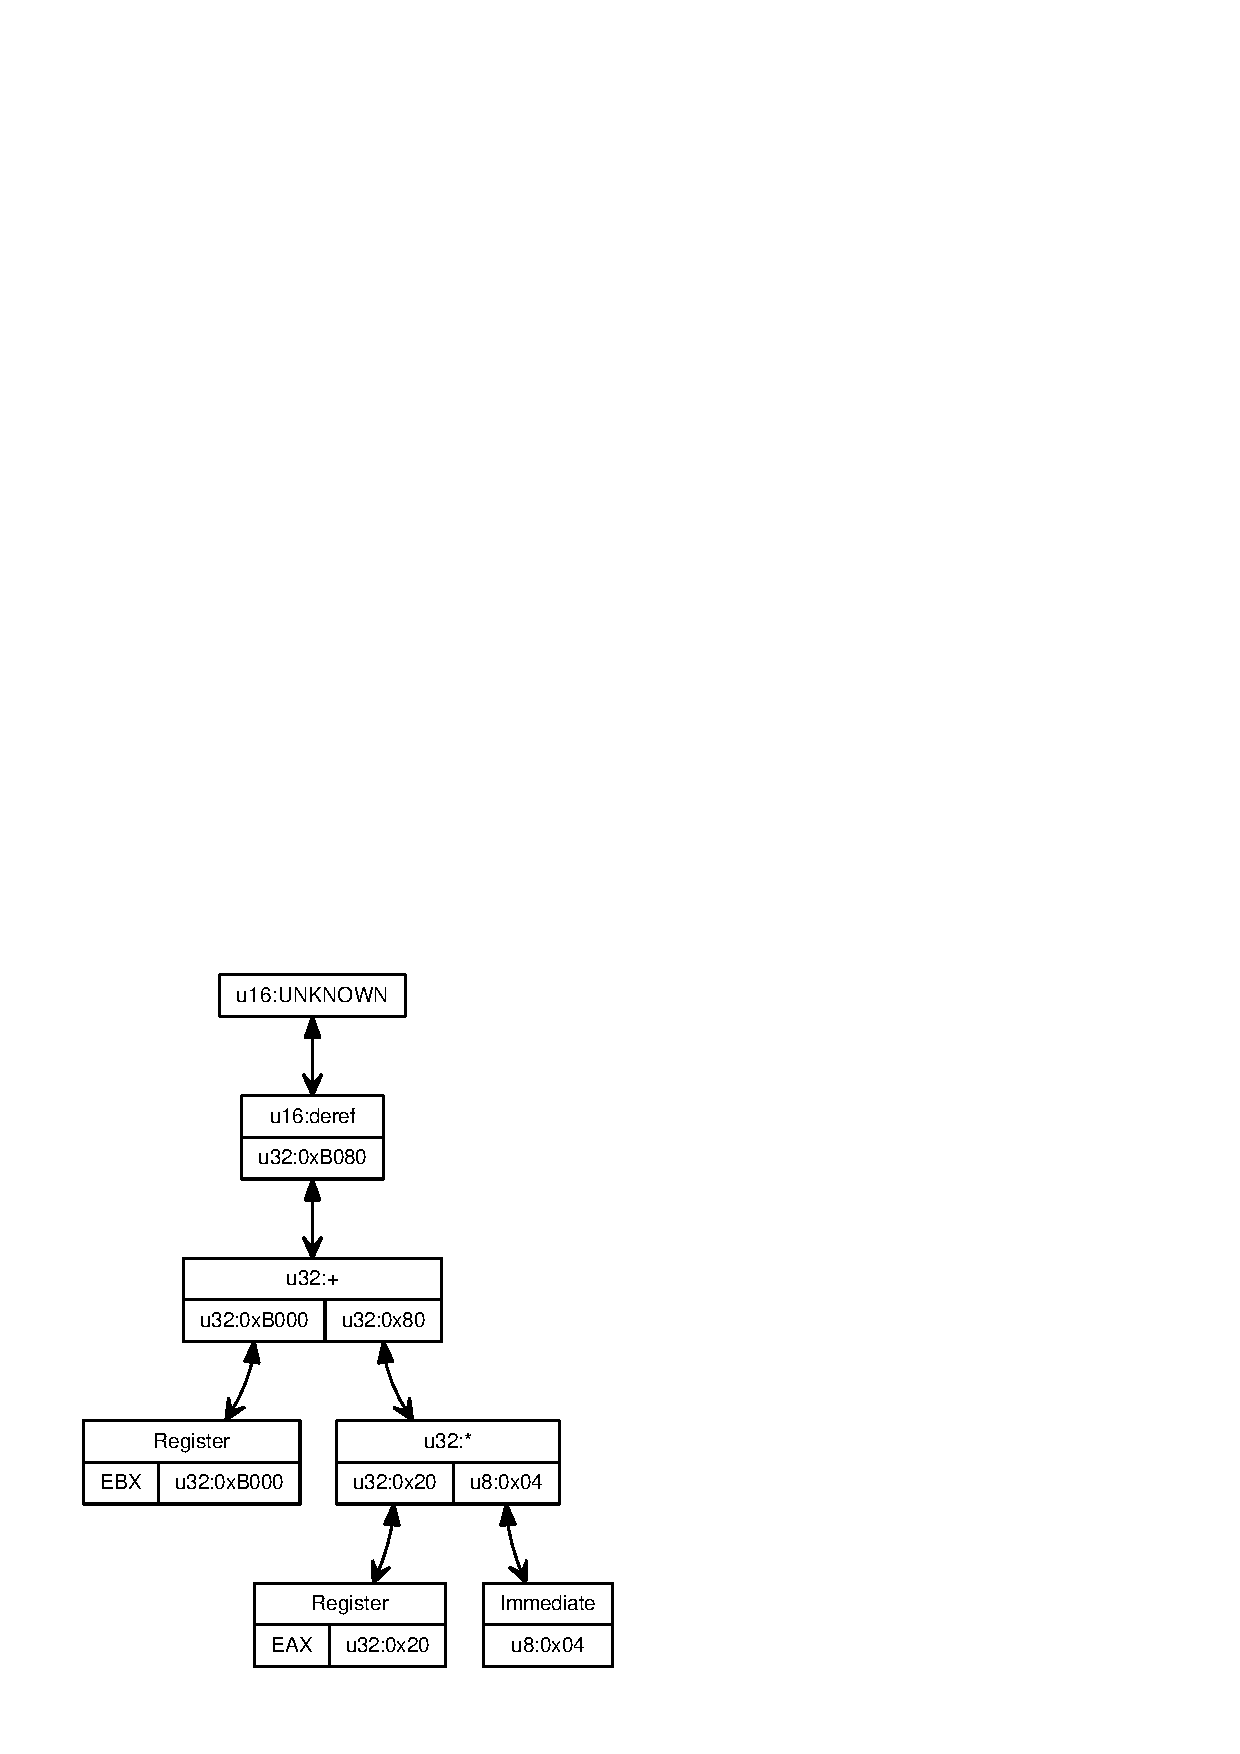
\includegraphics{deref-eval}
\caption{Applying {\ttfamily eval} to a Dereference tree with}
\end{DoxyImage}
 the state of the registers known and the state of memory unknown" 

\subsubsection{Member Functions}
\index{Dyninst::InstructionAPI::Expression@{Dyninst::InstructionAPI::Expression}!setValue@{setValue}}
\index{setValue@{setValue}!Dyninst::InstructionAPI::Expression@{Dyninst::InstructionAPI::Expression}}
\paragraph[{setValue}]{\setlength{\rightskip}{0pt plus 5cm}void setValue (
\begin{DoxyParamCaption}
\item[{const {\textbf Result} \&}]{ knownValue}
\end{DoxyParamCaption}
)}\hfill\label{classDyninst_1_1InstructionAPI_1_1Expression_a380c0c16c0c7ae2b83d1e7e603793cf2}

\begin{DoxyParams}{Parameters}
\item[{\em knownValue}]Sets the result of {\ttfamily eval} for this Expression to {\ttfamily knownValue} \end{DoxyParams}
\index{Dyninst::InstructionAPI::Expression@{Dyninst::InstructionAPI::Expression}!clearValue@{clearValue}}
\index{clearValue@{clearValue}!Dyninst::InstructionAPI::Expression@{Dyninst::InstructionAPI::Expression}}
\paragraph[{clearValue}]{\setlength{\rightskip}{0pt plus 5cm}void clearValue (
\begin{DoxyParamCaption}
{}
\end{DoxyParamCaption}
)}\hfill\label{classDyninst_1_1InstructionAPI_1_1Expression_a6b25a6f5cc0bd509a99eac0ee53f60b5}
{\ttfamily clearValue} sets the contents of this Expression to undefined. The next time {\ttfamily eval} is called, it will recalculate the value of the Expression. \index{Dyninst::InstructionAPI::Expression@{Dyninst::InstructionAPI::Expression}!bind@{bind}}
\index{bind@{bind}!Dyninst::InstructionAPI::Expression@{Dyninst::InstructionAPI::Expression}}
\paragraph[{bind}]{\setlength{\rightskip}{0pt plus 5cm}bool bind (
\begin{DoxyParamCaption}
\item[{{\textbf Expression} $\ast$}]{ expr, }
\item[{const {\textbf Result} \&}]{ value}
\end{DoxyParamCaption}
)\hspace{0.3cm}{\ttfamily  [virtual]}}\hfill\label{classDyninst_1_1InstructionAPI_1_1Expression_ad7949968db774d3d3539ecc5796772b8}
{\ttfamily bind} searches for all instances of the Expression {\ttfamily expr} within this Expression, and sets the result of {\ttfamily eval} for those subexpressions to {\ttfamily value}. {\ttfamily bind} returns true if at least one instance of {\ttfamily expr} was found in this Expression.

{\ttfamily bind} does not operate on subexpressions that happen to evaluate to the same value. For example, if a dereference of 0xDEADBEEF is bound to 0, and a register is bound to 0xDEADBEEF, a dereference of that register is not bound to 0. \index{Dyninst::InstructionAPI::Expression@{Dyninst::InstructionAPI::Expression}!apply@{apply}}
\index{apply@{apply}!Dyninst::InstructionAPI::Expression@{Dyninst::InstructionAPI::Expression}}
\paragraph[{apply}]{\setlength{\rightskip}{0pt plus 5cm}virtual void apply (
\begin{DoxyParamCaption}
\item[{Visitor $\ast$}]{}
\end{DoxyParamCaption}
)\hspace{0.3cm}{\ttfamily  [virtual]}}\hfill\label{classDyninst_1_1InstructionAPI_1_1Expression_aaef3bea3ba2584161f83b2ced7ef505b}
{\ttfamily apply} applies a Visitor to this expression. Visitors perform postfix-\/order traversal of the ASTs represented by an Expression, with user-\/defined actions performed at each node of the tree. \index{Dyninst::InstructionAPI::Expression@{Dyninst::InstructionAPI::Expression}!getChildren@{getChildren}}
\index{getChildren@{getChildren}!Dyninst::InstructionAPI::Expression@{Dyninst::InstructionAPI::Expression}}
\paragraph[{getChildren}]{\setlength{\rightskip}{0pt plus 5cm}virtual void getChildren (
\begin{DoxyParamCaption}
\item[{std::vector$<$ {\textbf Expression::Ptr} $>$ \&}]{ children}
\end{DoxyParamCaption}
) const\hspace{0.3cm}{\ttfamily  [pure virtual]}}\hfill\label{classDyninst_1_1InstructionAPI_1_1Expression_a6a1e1e53d272ca536170f3bdc95d9bdb}
{\ttfamily getChildren} may be called on an Expression taking a vector of ExpressionPtrs, rather than InstructionASTPtrs. All children which are Expressions will be appended to {\ttfamily children}. 
\subsection{Result Class}
\label{classDyninst_1_1InstructionAPI_1_1Result}\index{Dyninst::InstructionAPI::Result@{Dyninst::InstructionAPI::Result}}
\subsubsection*{Public Member Functions}
\begin{DoxyCompactItemize}
\item 
{\textbf Result} (Result\_\-Type t)
\item 
{\footnotesize template$<$typename T $>$ }\\{\textbf Result} (Result\_\-Type t, T v)
\item 
bool {\textbf operator==} (const {\textbf Result} \&o) const 
\item 
std::string {\textbf format} () const 
\end{DoxyCompactItemize}



A Result object represents a value computed by a Expression AST.

The Result class is a tagged-\/union representation of the results that Expressions can produce. It includes 8, 16, 32, 48, and 64 bit integers (signed and unsigned), bit values, and single and double precision floating point values. For each of these types, the value of a Result may be undefined, or it may be a value within the range of the type.

The {\ttfamily type} field is an enum that may contain any of the following values:
\begin{DoxyItemize}
\item {\ttfamily u8:} an unsigned 8-\/bit integer
\item {\ttfamily s8:} a signed 8-\/bit integer
\item {\ttfamily u16:} an unsigned 16-\/bit integer
\item {\ttfamily s16:} a signed 16-\/bit integer
\item {\ttfamily u32:} an unsigned 32-\/bit integer
\item {\ttfamily s32:} a signed 32-\/bit integer
\item {\ttfamily u48:} an unsigned 48-\/bit integer (IA32 pointers)
\item {\ttfamily s48:} a signed 48-\/bit integer (IA32 pointers)
\item {\ttfamily u64:} an unsigned 64-\/bit integer
\item {\ttfamily s64:} a signed 64-\/bit integer
\item {\ttfamily sp\_\-float:} a single-\/precision float
\item {\ttfamily dp\_\-float:} a double-\/precision float
\item {\ttfamily bit\_\-flag:} a single bit (individual flags)
\item {\ttfamily m512:} a 512-\/bit memory value
\item {\ttfamily dbl128:} a 128-\/bit integer, which often contains packed floating point values -\/ {\ttfamily m14:} a 14 byte memory value 
\end{DoxyItemize}

\subsubsection{Constructors \& Destructors}
\index{Dyninst::InstructionAPI::Result@{Dyninst::InstructionAPI::Result}!Result@{Result}}
\index{Result@{Result}!Dyninst::InstructionAPI::Result@{Dyninst::InstructionAPI::Result}}
\paragraph[{Result}]{\setlength{\rightskip}{0pt plus 5cm}{\textbf Result} (
\begin{DoxyParamCaption}
\item[{Result\_\-Type}]{ t}
\end{DoxyParamCaption}
)}\hfill\label{classDyninst_1_1InstructionAPI_1_1Result_a4236c02982253270277fa8053f52f0ea}
A Result may be constructed from a type without providing a value. This constructor creates a Result of type {\ttfamily t} with undefined contents. \index{Dyninst::InstructionAPI::Result@{Dyninst::InstructionAPI::Result}!Result@{Result}}
\index{Result@{Result}!Dyninst::InstructionAPI::Result@{Dyninst::InstructionAPI::Result}}
\paragraph[{Result}]{\setlength{\rightskip}{0pt plus 5cm}{\textbf Result} (
\begin{DoxyParamCaption}
\item[{Result\_\-Type}]{ t, }
\item[{T}]{ v}
\end{DoxyParamCaption}
)}\hfill\label{classDyninst_1_1InstructionAPI_1_1Result_a809c07cef0910505b40d9285f8c1af75}
A Result may be constructed from a type and any value convertible to the type that the tag represents. This constructor creates a Result of type {\ttfamily t} and contents {\ttfamily v} for any {\ttfamily v} that is implicitly convertible to type {\ttfamily t}. Attempting to construct a Result with a value that is incompatible with its type will result in a compile-\/time error. 

\subsubsection{Member Functions}
\index{Dyninst::InstructionAPI::Result@{Dyninst::InstructionAPI::Result}!operator==@{operator==}}
\index{operator==@{operator==}!Dyninst::InstructionAPI::Result@{Dyninst::InstructionAPI::Result}}
\paragraph[{operator==}]{\setlength{\rightskip}{0pt plus 5cm}bool operator== (
\begin{DoxyParamCaption}
\item[{const {\textbf Result} \&}]{ o}
\end{DoxyParamCaption}
) const}\hfill\label{classDyninst_1_1InstructionAPI_1_1Result_ac0d0c7ccdb0d1fa503b550460682ed5f}
Two Results are equal if any of the following hold:
\begin{DoxyItemize}
\item Both Results are of the same type and undefined
\item Both Results are of the same type, defined, and have the same value
\end{DoxyItemize}

Otherwise, they are unequal (due to having different types, an undefined Result compared to a defined Result, or different values). \index{Dyninst::InstructionAPI::Result@{Dyninst::InstructionAPI::Result}!format@{format}}
\index{format@{format}!Dyninst::InstructionAPI::Result@{Dyninst::InstructionAPI::Result}}
\paragraph[{format}]{\setlength{\rightskip}{0pt plus 5cm}std::string format (
\begin{DoxyParamCaption}
{}
\end{DoxyParamCaption}
) const}\hfill\label{classDyninst_1_1InstructionAPI_1_1Result_a204c75f752ee13cb64ccc2b7af3f687c}
Results are formatted as strings containing their contents, represented as hexadecimal. The type of the Result is not included in the output. 
\subsection{RegisterAST Class}
\label{classDyninst_1_1InstructionAPI_1_1RegisterAST}\index{Dyninst::InstructionAPI::RegisterAST@{Dyninst::InstructionAPI::RegisterAST}}
\subsubsection*{Public Member Functions}
\begin{DoxyCompactItemize}
\item 
virtual void {\textbf getChildren} (vector$<$ InstructionAST::Ptr $>$ \&children) const 
\item 
virtual void {\textbf getUses} (set$<$ InstructionAST::Ptr $>$ \&uses)
\item 
virtual bool {\textbf isUsed} (InstructionAST::Ptr findMe) const 
\item 
bool {\textbf operator$<$} (const {\textbf RegisterAST} \&rhs) const 
\end{DoxyCompactItemize}
\subsubsection*{Static Public Member Functions}
\begin{DoxyCompactItemize}
\item 
static {\textbf RegisterAST} {\textbf makePC} (Dyninst::Architecture arch)
\item 
static {\textbf RegisterAST::Ptr} {\textbf promote} (const InstructionAST::Ptr reg)
\end{DoxyCompactItemize}



A RegisterAST object represents a register contained in an operand. As a RegisterAST is a Expression, it may contain the physical register's contents if they are known. 

\subsubsection{Member Functions}
\index{Dyninst::InstructionAPI::RegisterAST@{Dyninst::InstructionAPI::RegisterAST}!getChildren@{getChildren}}
\index{getChildren@{getChildren}!Dyninst::InstructionAPI::RegisterAST@{Dyninst::InstructionAPI::RegisterAST}}
\paragraph[{getChildren}]{\setlength{\rightskip}{0pt plus 5cm}void getChildren (
\begin{DoxyParamCaption}
\item[{vector$<$ InstructionAST::Ptr $>$ \&}]{ children}
\end{DoxyParamCaption}
) const\hspace{0.3cm}{\ttfamily  [virtual]}}\hfill\label{classDyninst_1_1InstructionAPI_1_1RegisterAST_abd80c13b7e8fa7952220858b72b15c14}
By definition, a RegisterAST object has no children. 
\begin{DoxyParams}{Parameters}
\item[{\em children}]Since a RegisterAST has no children, the {\ttfamily children} parameter is unchanged by this method. \end{DoxyParams}



\index{Dyninst::InstructionAPI::RegisterAST@{Dyninst::InstructionAPI::RegisterAST}!getUses@{getUses}}
\index{getUses@{getUses}!Dyninst::InstructionAPI::RegisterAST@{Dyninst::InstructionAPI::RegisterAST}}
\paragraph[{getUses}]{\setlength{\rightskip}{0pt plus 5cm}void getUses (
\begin{DoxyParamCaption}
\item[{set$<$ InstructionAST::Ptr $>$ \&}]{ uses}
\end{DoxyParamCaption}
)\hspace{0.3cm}{\ttfamily  [virtual]}}\hfill\label{classDyninst_1_1InstructionAPI_1_1RegisterAST_a82c5ae077a4ab1bd306104ae784c73ee}
By definition, the use set of a RegisterAST object is itself. 
\begin{DoxyParams}{Parameters}
\item[{\em uses}]This RegisterAST will be inserted into {\ttfamily uses}. \end{DoxyParams}



\index{Dyninst::InstructionAPI::RegisterAST@{Dyninst::InstructionAPI::RegisterAST}!isUsed@{isUsed}}
\index{isUsed@{isUsed}!Dyninst::InstructionAPI::RegisterAST@{Dyninst::InstructionAPI::RegisterAST}}
\paragraph[{isUsed}]{\setlength{\rightskip}{0pt plus 5cm}bool isUsed (
\begin{DoxyParamCaption}
\item[{InstructionAST::Ptr}]{ findMe}
\end{DoxyParamCaption}
) const\hspace{0.3cm}{\ttfamily  [virtual]}}\hfill\label{classDyninst_1_1InstructionAPI_1_1RegisterAST_a71169e7bb9813302ddc3486c3d9eb65d}
{\ttfamily isUsed} returns true if {\ttfamily findMe} is a RegisterAST that represents the same register as this RegisterAST, and false otherwise. 


\index{Dyninst::InstructionAPI::RegisterAST@{Dyninst::InstructionAPI::RegisterAST}!makePC@{makePC}}
\index{makePC@{makePC}!Dyninst::InstructionAPI::RegisterAST@{Dyninst::InstructionAPI::RegisterAST}}
\paragraph[{makePC}]{\setlength{\rightskip}{0pt plus 5cm}{\textbf RegisterAST} makePC (
\begin{DoxyParamCaption}
\item[{Dyninst::Architecture}]{ arch}
\end{DoxyParamCaption}
)\hspace{0.3cm}{\ttfamily  [static]}}\hfill\label{classDyninst_1_1InstructionAPI_1_1RegisterAST_aafa5d5b65d94a4555ac944fa5f695007}
Utility function to get a Register object that represents the program counter.

{\ttfamily makePC} is provided to support platform-\/independent control flow analysis. \index{Dyninst::InstructionAPI::RegisterAST@{Dyninst::InstructionAPI::RegisterAST}!operator$<$@{operator$<$}}
\index{operator$<$@{operator$<$}!Dyninst::InstructionAPI::RegisterAST@{Dyninst::InstructionAPI::RegisterAST}}
\paragraph[{operator$<$}]{\setlength{\rightskip}{0pt plus 5cm}bool operator$<$ (
\begin{DoxyParamCaption}
\item[{const {\textbf RegisterAST} \&}]{ rhs}
\end{DoxyParamCaption}
) const}\hfill\label{classDyninst_1_1InstructionAPI_1_1RegisterAST_ad043f2b4d3c8bee6ea00995f4ad5fb33}
We define a partial ordering on registers by their register number so that they may be placed into sets or other sorted containers. \index{Dyninst::InstructionAPI::RegisterAST@{Dyninst::InstructionAPI::RegisterAST}!promote@{promote}}
\index{promote@{promote}!Dyninst::InstructionAPI::RegisterAST@{Dyninst::InstructionAPI::RegisterAST}}
\paragraph[{promote}]{\setlength{\rightskip}{0pt plus 5cm}{\textbf RegisterAST::Ptr} promote (
\begin{DoxyParamCaption}
\item[{const InstructionAST::Ptr}]{ reg}
\end{DoxyParamCaption}
)\hspace{0.3cm}{\ttfamily  [static]}}\hfill\label{classDyninst_1_1InstructionAPI_1_1RegisterAST_a012fdc0ebb54d7d552b0d3a87f4107ca}
Utility function to hide aliasing complexity on platforms (IA-\/32) that allow addressing part or all of a register 
\subsection{Immediate Class}
\label{classDyninst_1_1InstructionAPI_1_1Immediate}\index{Dyninst::InstructionAPI::Immediate@{Dyninst::InstructionAPI::Immediate}}
\subsubsection*{Public Member Functions}
\begin{DoxyCompactItemize}
\item 
virtual bool {\textbf isUsed} (InstructionAST::Ptr findMe) const 
\end{DoxyCompactItemize}



The Immediate class represents an immediate value in an operand

Since an Immediate represents a constant value, the {\ttfamily setValue} and {\ttfamily clearValue} interface are disabled on Immediate objects. If an immediate value is being modified, a new Immediate object should be created to represent the new value. 

\subsubsection{Member Functions}
\index{Dyninst::InstructionAPI::Immediate@{Dyninst::InstructionAPI::Immediate}!isUsed@{isUsed}}
\index{isUsed@{isUsed}!Dyninst::InstructionAPI::Immediate@{Dyninst::InstructionAPI::Immediate}}
\paragraph[{isUsed}]{\setlength{\rightskip}{0pt plus 5cm}bool isUsed (
\begin{DoxyParamCaption}
\item[{InstructionAST::Ptr}]{ findMe}
\end{DoxyParamCaption}
) const\hspace{0.3cm}{\ttfamily  [virtual]}}\hfill\label{classDyninst_1_1InstructionAPI_1_1Immediate_a71169e7bb9813302ddc3486c3d9eb65d}
{\ttfamily isUsed}, when called on an Immediate, will return true if {\ttfamily findMe} represents an Immediate with the same value. While this convention may seem arbitrary, it allows {\ttfamily isUsed} to follow a natural rule: an InstructionAST is used by another InstructionAST if and only if the first InstructionAST is a subtree of the second one. 



\subsection{BinaryFunction Class}
\label{classDyninst_1_1InstructionAPI_1_1BinaryFunction}\index{Dyninst::InstructionAPI::BinaryFunction@{Dyninst::InstructionAPI::BinaryFunction}}
\subsubsection*{Public Member Functions}
\begin{DoxyCompactItemize}
\item 
{\textbf BinaryFunction} ({\textbf Expression::Ptr} arg1, {\textbf Expression::Ptr} arg2, Result\_\-Type result\_\-type, funcT::Ptr func)
\item 
virtual const {\textbf Result} \& {\textbf eval} () const 
\item 
virtual void {\textbf getChildren} (vector$<$ InstructionAST::Ptr $>$ \&children) const 
\item 
virtual void {\textbf getUses} (set$<$ InstructionAST::Ptr $>$ \&uses)
\item 
virtual bool {\textbf isUsed} (InstructionAST::Ptr findMe) const 
\end{DoxyCompactItemize}



A BinaryFunction object represents a function that can combine two Expressions and produce another ValueComputation.

For the purposes of representing a single operand of an instruction, the BinaryFunctions of interest are addition and multiplication of integer values; this allows a Expression to represent all addressing modes on the architectures currently supported by the Instruction API. 

\subsubsection{Constructors \& Destructors}
\index{Dyninst::InstructionAPI::BinaryFunction@{Dyninst::InstructionAPI::BinaryFunction}!BinaryFunction@{BinaryFunction}}
\index{BinaryFunction@{BinaryFunction}!Dyninst::InstructionAPI::BinaryFunction@{Dyninst::InstructionAPI::BinaryFunction}}
\paragraph[{BinaryFunction}]{\setlength{\rightskip}{0pt plus 5cm}{\textbf BinaryFunction} (
\begin{DoxyParamCaption}
\item[{{\textbf Expression::Ptr}}]{ arg1, }
\item[{{\textbf Expression::Ptr}}]{ arg2, }
\item[{Result\_\-Type}]{ result\_\-type, }
\item[{funcT::Ptr}]{ func}
\end{DoxyParamCaption}
)}\hfill\label{classDyninst_1_1InstructionAPI_1_1BinaryFunction_ac1d9ee9e075b29690d4f1f17949d94d0}

\begin{DoxyParams}{Parameters}
\item[{\em arg1}]first input to function \item[{\em arg2}]second input to function \item[{\em result\_\-type}]type of the function's result \item[{\em func}]implementation of the function\end{DoxyParams}
The constructor for a BinaryFunction may take a reference-\/counted pointer or a plain C++ pointer to each of the child Expressions that represent its arguments. Since the reference-\/counted implementation requires explicit construction, we provide overloads for all four combinations of plain and reference-\/counted pointers. Note that regardless of which constructor is used, the pointers {\ttfamily arg1} and {\ttfamily arg2} become owned by the BinaryFunction being constructed, and should not be deleted. They will be cleaned up when the BinaryFunction object is destroyed.

The {\ttfamily func} parameter is a binary functor on two Results. It should be derived from {\ttfamily funcT}. {\ttfamily addResult} and {\ttfamily multResult}, which respectively add and multiply two Results, are provided as part of the InstructionAPI, as they are necessary for representing address calculations. Other {\ttfamily funcTs} may be implemented by the user if desired. funcTs have names associated with them for output and debugging purposes. The addition and multiplication functors provided with the Instruction API are named \char`\"{}+\char`\"{} and \char`\"{}$\ast$\char`\"{}, respectively. 

\subsubsection{Member Functions}
\index{Dyninst::InstructionAPI::BinaryFunction@{Dyninst::InstructionAPI::BinaryFunction}!eval@{eval}}
\index{eval@{eval}!Dyninst::InstructionAPI::BinaryFunction@{Dyninst::InstructionAPI::BinaryFunction}}
\paragraph[{eval}]{\setlength{\rightskip}{0pt plus 5cm}const {\textbf Result} \& eval (
\begin{DoxyParamCaption}
{}
\end{DoxyParamCaption}
) const\hspace{0.3cm}{\ttfamily  [virtual]}}\hfill\label{classDyninst_1_1InstructionAPI_1_1BinaryFunction_a9d6e92c2e65bf1162faa3734911ebff3}
The BinaryFunction version of {\ttfamily eval} allows the {\ttfamily eval} mechanism to handle complex addressing modes. Like all of the ValueComputation implementations, a BinaryFunction's {\ttfamily eval} will return the result of evaluating the expression it represents if possible, or an empty Result otherwise. A BinaryFunction may have arguments that can be evaluated, or arguments that cannot. Additionally, it may have a real function pointer, or it may have a null function pointer. If the arguments can be evaluated and the function pointer is real, a result other than an empty Result is guaranteed to be returned. This result is cached after its initial calculation; the caching mechanism also allows outside information to override the results of the BinaryFunction's internal computation. If the cached result exists, it is guaranteed to be returned even if the arguments or the function are not evaluable. 


\index{Dyninst::InstructionAPI::BinaryFunction@{Dyninst::InstructionAPI::BinaryFunction}!getChildren@{getChildren}}
\index{getChildren@{getChildren}!Dyninst::InstructionAPI::BinaryFunction@{Dyninst::InstructionAPI::BinaryFunction}}
\paragraph[{getChildren}]{\setlength{\rightskip}{0pt plus 5cm}virtual void getChildren (
\begin{DoxyParamCaption}
\item[{vector$<$ InstructionAST::Ptr $>$ \&}]{ children}
\end{DoxyParamCaption}
) const\hspace{0.3cm}{\ttfamily  [virtual]}}\hfill\label{classDyninst_1_1InstructionAPI_1_1BinaryFunction_adabe6006766a7aaa6fa099f5f0ca5c0c}
The children of a BinaryFunction are its two arguments. 
\begin{DoxyParams}{Parameters}
\item[{\em children}]Appends the children of this BinaryFunction to {\ttfamily children}. \end{DoxyParams}



\index{Dyninst::InstructionAPI::BinaryFunction@{Dyninst::InstructionAPI::BinaryFunction}!getUses@{getUses}}
\index{getUses@{getUses}!Dyninst::InstructionAPI::BinaryFunction@{Dyninst::InstructionAPI::BinaryFunction}}
\paragraph[{getUses}]{\setlength{\rightskip}{0pt plus 5cm}virtual void getUses (
\begin{DoxyParamCaption}
\item[{set$<$ InstructionAST::Ptr $>$ \&}]{ uses}
\end{DoxyParamCaption}
)\hspace{0.3cm}{\ttfamily  [virtual]}}\hfill\label{classDyninst_1_1InstructionAPI_1_1BinaryFunction_a3793407f71d4fba12ae0af46e78da4b4}
The use set of a BinaryFunction is the union of the use sets of its children. 
\begin{DoxyParams}{Parameters}
\item[{\em uses}]Appends the use set of this BinaryFunction to {\ttfamily uses}. \end{DoxyParams}



\index{Dyninst::InstructionAPI::BinaryFunction@{Dyninst::InstructionAPI::BinaryFunction}!isUsed@{isUsed}}
\index{isUsed@{isUsed}!Dyninst::InstructionAPI::BinaryFunction@{Dyninst::InstructionAPI::BinaryFunction}}
\paragraph[{isUsed}]{\setlength{\rightskip}{0pt plus 5cm}virtual bool isUsed (
\begin{DoxyParamCaption}
\item[{InstructionAST::Ptr}]{ findMe}
\end{DoxyParamCaption}
) const\hspace{0.3cm}{\ttfamily  [virtual]}}\hfill\label{classDyninst_1_1InstructionAPI_1_1BinaryFunction_af5b1db3ca39797ac0f619e04dd8bf9fc}
{\ttfamily isUsed} returns true if {\ttfamily findMe} is an argument of this BinaryFunction, or if it is in the use set of either argument. 



\subsection{Dereference Class}
\label{classDyninst_1_1InstructionAPI_1_1Dereference}\index{Dyninst::InstructionAPI::Dereference@{Dyninst::InstructionAPI::Dereference}}
\subsubsection*{Public Member Functions}
\begin{DoxyCompactItemize}
\item 
{\textbf Dereference} ({\textbf Expression::Ptr} addr, Result\_\-Type result\_\-type)
\item 
virtual void {\textbf getChildren} (vector$<$ InstructionAST::Ptr $>$ \&children) const 
\item 
virtual void {\textbf getUses} (set$<$ InstructionAST::Ptr $>$ \&uses)
\item 
virtual bool {\textbf isUsed} (InstructionAST::Ptr findMe) const 
\end{DoxyCompactItemize}



A Dereference object is a Expression that dereferences another ValueComputation.

A Dereference contains an Expression representing an effective address computation. Its use set is the same as the use set of the Expression being dereferenced.

It is not possible, given the information in a single instruction, to evaluate the result of a dereference. {\ttfamily eval} may still be called on a Expression that includes dereferences, but the expected use case is as follows:
\begin{DoxyItemize}
\item Determine the address being used in a dereference via the {\ttfamily eval} mechanism
\item Perform analysis to determine the contents of that address
\item If necessary, fill in the Dereference node with the contents of that addresss, using {\ttfamily setValue} 
\end{DoxyItemize}

The type associated with a Dereference node will be the type of the value {\itshape read\/} {\itshape from\/} {\itshape memory\/}, not the type used for the address computation. Two Dereferences that access the same address but interpret the contents of that memory as different types will produce different values. The children of a Dereference at a given address are identical, regardless of the type of dereference being performed at that address. For example, the Expression shown in Figure 6 could have its root Dereference, which interprets the memory being dereferenced as a unsigned 16-\/bit integer, replaced with a Dereference that interprets the memory being dereferenced as any other type. The remainder of the Expression tree would, however, remain unchanged. 

\subsubsection{Constructors \& Destructors}
\index{Dyninst::InstructionAPI::Dereference@{Dyninst::InstructionAPI::Dereference}!Dereference@{Dereference}}
\index{Dereference@{Dereference}!Dyninst::InstructionAPI::Dereference@{Dyninst::InstructionAPI::Dereference}}
\paragraph[{Dereference}]{\setlength{\rightskip}{0pt plus 5cm}{\textbf Dereference} (
\begin{DoxyParamCaption}
\item[{{\textbf Expression::Ptr}}]{ addr, }
\item[{Result\_\-Type}]{ result\_\-type}
\end{DoxyParamCaption}
)}\hfill\label{classDyninst_1_1InstructionAPI_1_1Dereference_a39fee3d3fdcb936e63f9e64f250cd889}
A Dereference is constructed from a Expression pointer (raw or shared) representing the address to be dereferenced and a type indicating how the memory at the address in question is to be interpreted. 

\subsubsection{Member Functions}
\index{Dyninst::InstructionAPI::Dereference@{Dyninst::InstructionAPI::Dereference}!getChildren@{getChildren}}
\index{getChildren@{getChildren}!Dyninst::InstructionAPI::Dereference@{Dyninst::InstructionAPI::Dereference}}
\paragraph[{getChildren}]{\setlength{\rightskip}{0pt plus 5cm}virtual void getChildren (
\begin{DoxyParamCaption}
\item[{vector$<$ InstructionAST::Ptr $>$ \&}]{ children}
\end{DoxyParamCaption}
) const\hspace{0.3cm}{\ttfamily  [virtual]}}\hfill\label{classDyninst_1_1InstructionAPI_1_1Dereference_adabe6006766a7aaa6fa099f5f0ca5c0c}
A Dereference has one child, which represents the address being dereferenced. 
\begin{DoxyParams}{Parameters}
\item[{\em children}]Appends the child of this Dereference to {\ttfamily children}. \end{DoxyParams}



\index{Dyninst::InstructionAPI::Dereference@{Dyninst::InstructionAPI::Dereference}!getUses@{getUses}}
\index{getUses@{getUses}!Dyninst::InstructionAPI::Dereference@{Dyninst::InstructionAPI::Dereference}}
\paragraph[{getUses}]{\setlength{\rightskip}{0pt plus 5cm}virtual void getUses (
\begin{DoxyParamCaption}
\item[{set$<$ InstructionAST::Ptr $>$ \&}]{ uses}
\end{DoxyParamCaption}
)\hspace{0.3cm}{\ttfamily  [virtual]}}\hfill\label{classDyninst_1_1InstructionAPI_1_1Dereference_a3793407f71d4fba12ae0af46e78da4b4}
The use set of a Dereference is the same as the use set of its children. 
\begin{DoxyParams}{Parameters}
\item[{\em uses}]The use set of this Dereference is inserted into {\ttfamily uses}. \end{DoxyParams}



\index{Dyninst::InstructionAPI::Dereference@{Dyninst::InstructionAPI::Dereference}!isUsed@{isUsed}}
\index{isUsed@{isUsed}!Dyninst::InstructionAPI::Dereference@{Dyninst::InstructionAPI::Dereference}}
\paragraph[{isUsed}]{\setlength{\rightskip}{0pt plus 5cm}virtual bool isUsed (
\begin{DoxyParamCaption}
\item[{InstructionAST::Ptr}]{ findMe}
\end{DoxyParamCaption}
) const\hspace{0.3cm}{\ttfamily  [virtual]}}\hfill\label{classDyninst_1_1InstructionAPI_1_1Dereference_af5b1db3ca39797ac0f619e04dd8bf9fc}
An InstructionAST is used by a Dereference if it is equivalent to the Dereference or it is used by the lone child of the Dereference 



\subsection{RegInfo Struct}
\label{structDyninst_1_1InstructionAPI_1_1RegInfo}\index{Dyninst::InstructionAPI::RegInfo@{Dyninst::InstructionAPI::RegInfo}}


The RegInfo struct associates a register ID with its size and name.  



\subsection{IA32RegTable Struct}
\label{structDyninst_1_1InstructionAPI_1_1IA32RegTable}\index{Dyninst::InstructionAPI::IA32RegTable@{Dyninst::InstructionAPI::IA32RegTable}}


Register names for disassembly and debugging.  



\subsection{InstructionDecoder\_\-x86 Class}
\label{classDyninst_1_1InstructionAPI_1_1InstructionDecoder__x86}\index{Dyninst::InstructionAPI::InstructionDecoder\_\-x86@{Dyninst::InstructionAPI::InstructionDecoder\_\-x86}}



The InstructionDecoder class decodes instructions, given a buffer of bytes and a length, and constructs an Instruction. The InstructionDecoder will, by default, be constructed to decode machine language on the platform on which it has been compiled. The buffer will be treated as if there is an instruction stream starting at the beginning of the buffer. InstructionDecoder objects are given a buffer from which to decode at construction. Calls to {\ttfamily decode} will proceed to decode instructions sequentially from that buffer until its end is reached. At that point, all subsequent calls to {\ttfamily decode} will return an invalid Instruction object. An InstructionDecoder object may alternately be constructed without designating a buffer, and the buffer may be specified at the time {\ttfamily decode} is called. This method of use may be more convenient for users who are decoding non-\/contiguous instructions. 
\printindex
\end{document}
